\documentclass{beamer}

\usepackage[T1]{fontenc}
\usepackage{lmodern}
\usepackage{graphicx}
\usepackage{amsmath}
\usepackage{amssymb}
\usepackage{booktabs}
\usepackage{xcolor}
\usepackage{tikz}
\usepackage{array}
\usepackage{colortbl}
\usepackage[authoryear,round]{natbib}
\usepackage{ragged2e}

\usetheme{Madrid}
\usecolortheme{default}
\setbeamertemplate{navigation symbols}{}
\setbeamertemplate{footline}[frame number]
\setbeamersize{text margin left=0.6cm, text margin right=0.6cm}

\definecolor{myprimary}{HTML}{FF9D00}
\definecolor{mysecondary}{HTML}{FF8360}
\definecolor{mydark}{HTML}{243447}
\definecolor{mylight}{HTML}{FFF4E8}
\definecolor{mysoft}{HTML}{F7F7F7}

\setbeamercolor{structure}{fg=myprimary}
\setbeamercolor{title}{fg=white,bg=myprimary}
\setbeamercolor{subtitle}{fg=myprimary}
\setbeamercolor{frametitle}{fg=white,bg=myprimary!90}
\setbeamercolor{block title}{fg=white,bg=myprimary!85}
\setbeamercolor{block body}{fg=black,bg=mylight}
\setbeamercolor{normal text}{fg=mydark,bg=white}
\setbeamercolor{alerted text}{fg=mysecondary}

\setbeamerfont{title}{series=\bfseries,size=\Large}
\setbeamerfont{frametitle}{series=\bfseries,size=\large}
\setbeamerfont{block title}{series=\bfseries}
\setbeamertemplate{bibliography item}[text]
\setlength{\bibsep}{1pt plus 0.2ex}
\bibliographystyle{abbrvnat}

\newcommand{\lerobot}{\texttt{lerobot}}
\newcommand{\lerobotdataset}{\texttt{LeRobotDataset}}
\newcommand{\pizero}{\(\pi_0\)}
\newcommand{\highlight}[1]{\textcolor{myprimary}{\textbf{#1}}}
\newcommand{\statbox}[2]{%
  \begingroup
  \setlength{\fboxsep}{8pt}%
  \colorbox{mylight}{\parbox{\dimexpr\linewidth-2\fboxsep\relax}{\raggedright\textbf{\large #1}\\[-1pt]\small #2}}%
  \endgroup
}

\newcommand{\circled}[1]{%
  \tikz[baseline=(char.base)]\node[draw,circle,inner sep=1pt,thick](char){\textbf{#1}};%
}

\newcommand{\lightbox}[1]{%
  \tikz[baseline=(txt.base)]{
    \node[
      fill=myprimary!15,
      rounded corners=2pt,
      inner xsep=4pt,
      inner ysep=1.5pt
    ] (txt) {\strut #1};
  }%
}

\newcommand{\commonauthors}{%
  Francesco Capuano \and
  Caroline Pascal \and
  Adil Zouitine \and
  Thomas Wolf \and
  Michel Aractingi
}

\newcommand{\shortauthors}{%
  Francesco Capuano, Caroline Pascal, Adil Zouitine, Thomas Wolf, Michel Aractingi
}

\newcommand{\chaptertitleframe}[1]{%
  \begin{frame}[plain]
    \vspace{0.35cm}
    \begin{center}
      \begin{beamercolorbox}[wd=0.86\paperwidth,rounded=true,sep=10pt,center]{title}
        \usebeamerfont{title}\inserttitle
      \end{beamercolorbox}

      \vspace{0.55cm}
      {\Large\bfseries\textcolor{myprimary}{\insertsubtitle}\par}
      \vspace{0.15cm}
      {\small\color{mydark}\shortauthors\par}

      \vspace{0.45cm}
      
\includegraphics[height=1.0cm]{hf.pdf}
      \hspace{0.45cm}
      
\includegraphics[height=0.95cm]{oxford_logo.png}

      \vspace{0.55cm}
      \begin{beamercolorbox}[wd=0.8\paperwidth,rounded=true,sep=8pt,center]{block body}
        \small #1
      \end{beamercolorbox}
    \end{center}
  \end{frame}
}

\newcommand{\sources}[1]{%
  \vfill
  {\raggedright\tiny\color{black!65}\textbf{Refs:} #1\par}
}

\graphicspath{{../../../figures/}{../../../logos/}}

\title[Robot Learning Tutorial]{Robot Learning: A Tutorial}
\subtitle{Chapter 4: Robot Imitation Learning}
\author[Capuano et al.]{\commonauthors}
\date{}
\titlegraphic{
  \vspace{-1.1cm}
  
\includegraphics[height=1.4cm]{hf.pdf}
  \hspace{0.3cm}
  
\includegraphics[height=1.2cm]{oxford_logo.png}
}

\begin{document}

\chaptertitleframe{How behavioral cloning becomes practical in robotics once action generation is treated as a multimodal generative modeling problem.}

\begin{frame}{Roadmap}
  \begin{enumerate}
    \item Why behavioral cloning is attractive in robotics
    \item Why pointwise policies break
    \item Why generative models help
    \item ACT, Diffusion Policy, and optimized inference
  \end{enumerate}
\end{frame}

\begin{frame}{Why Imitation Learning Matters}
  \begin{itemize}
    \item Real-world RL is slowed down by exploration risk, resets, and reward engineering.
    \item Behavioral Cloning reframes control as \highlight{learning from expert demonstrations}.
    \item The dataset already encodes human intent, successful endpoints, and task preferences.
  \end{itemize}

  \vspace{0.2cm}
  \statbox{Main tradeoff}{BC avoids reward design and unsafe exploration, but it can only learn from the quality and coverage of the demonstrations it sees.}
\end{frame}

\begin{frame}{What Demonstration Data Looks Like}
  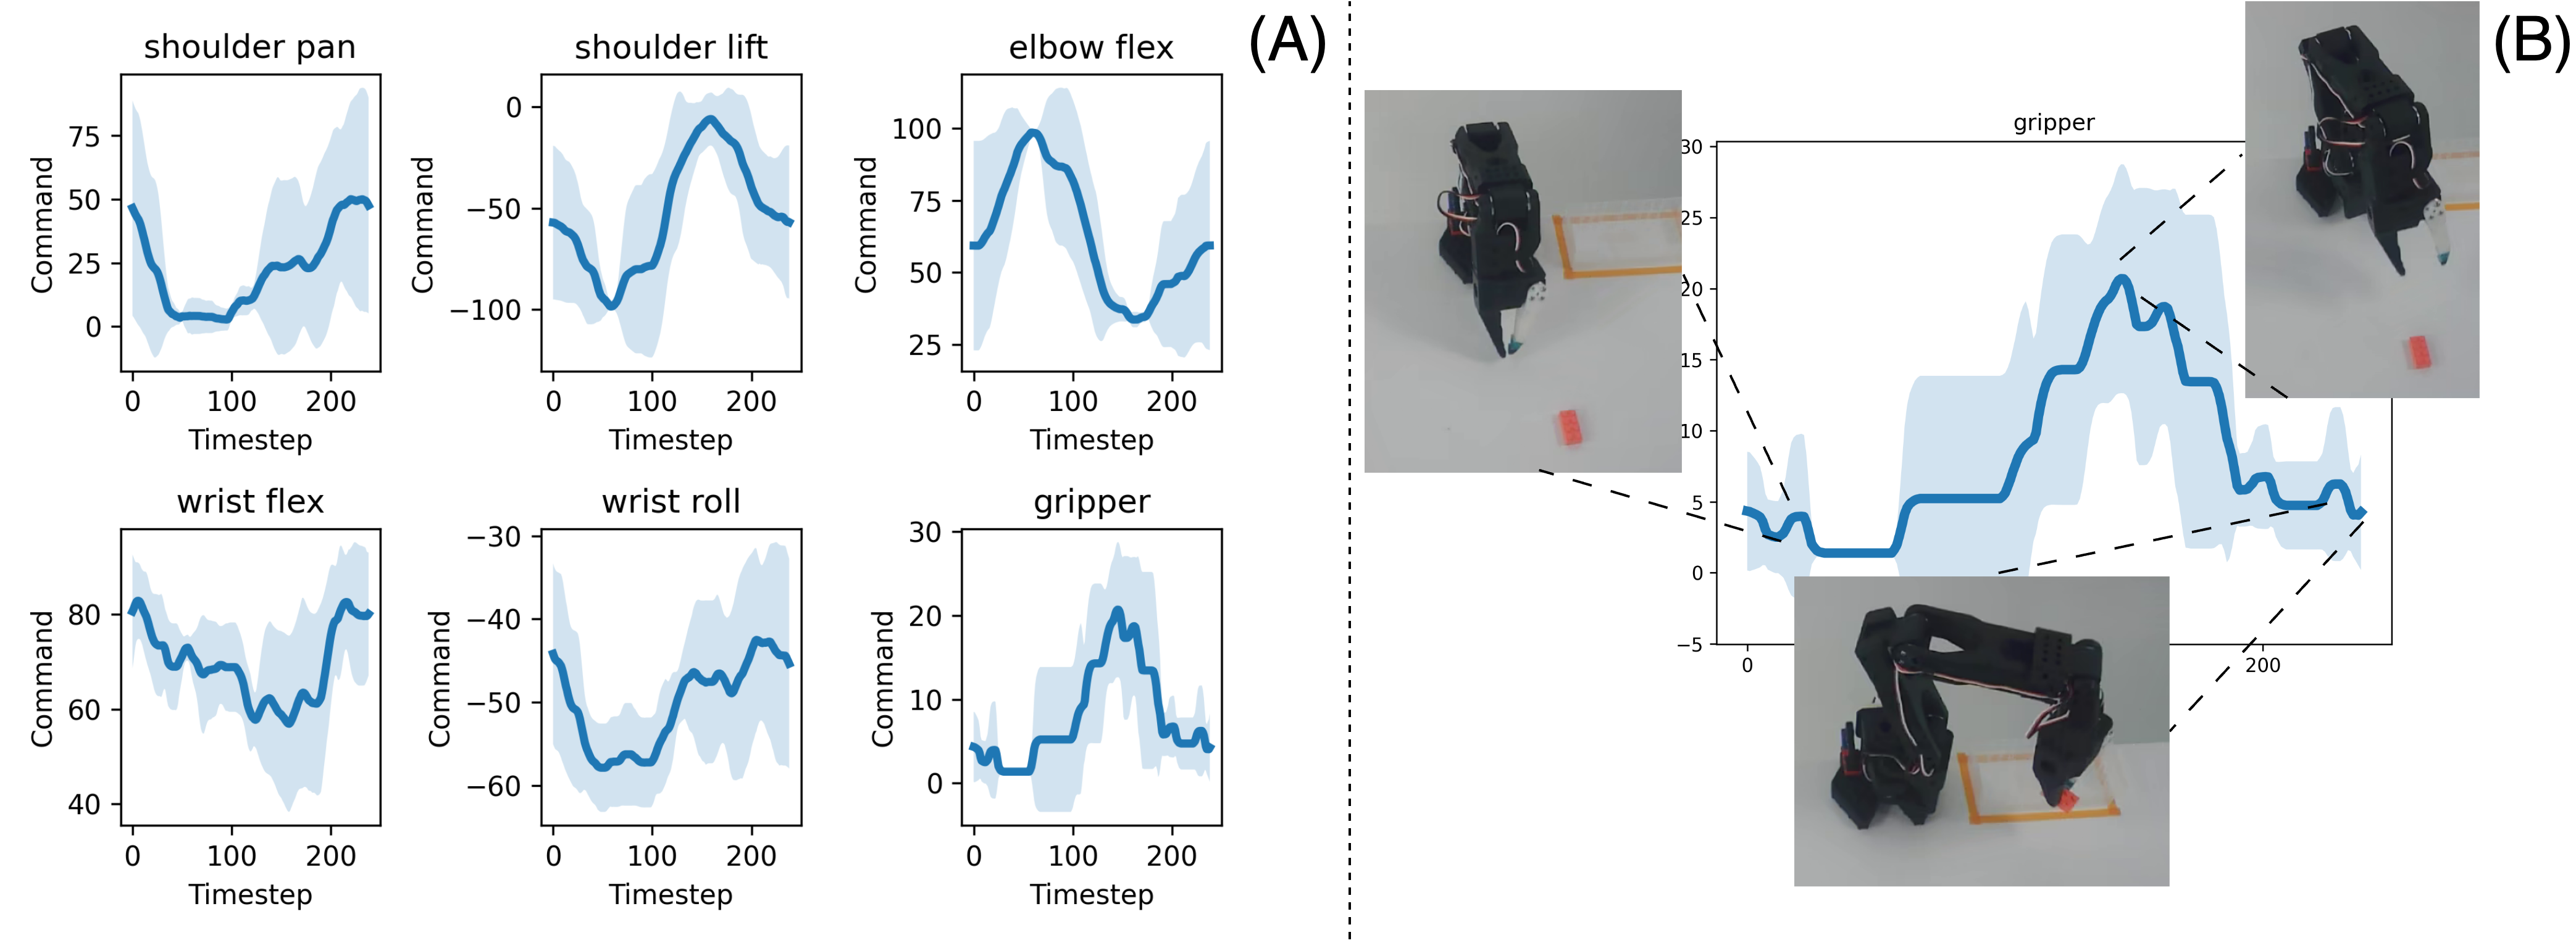
\includegraphics[width=\linewidth,height=0.68\textheight,keepaspectratio]{ch4/ch4-bc-trajectories.png}
  \begin{itemize}
    \item Trajectories combine \highlight{proprioception and camera streams} over time.
  \end{itemize}
\end{frame}

\begin{frame}{BC as Observation-to-Action Learning}
  \begin{columns}[T,onlytextwidth]
    \begin{column}{0.58\textwidth}
      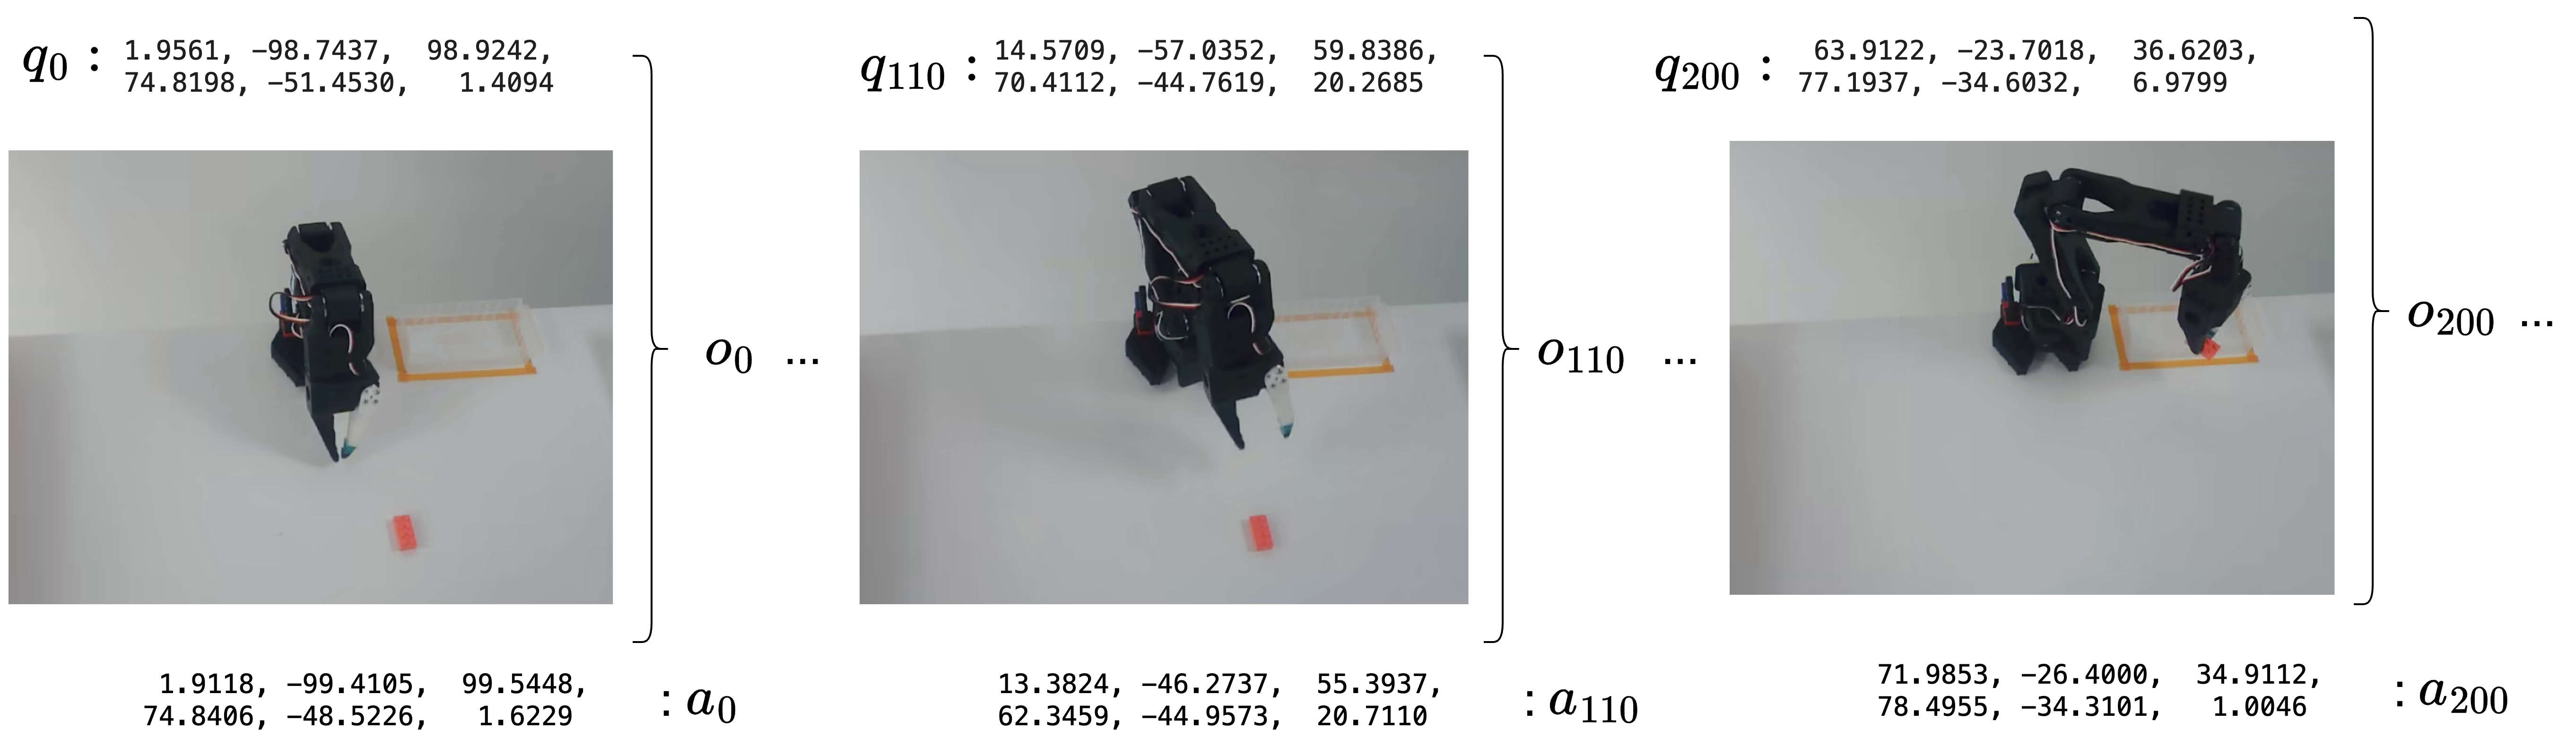
\includegraphics[width=\linewidth]{ch4/ch4-observation-action-mapping.png}
    \end{column}
    \begin{column}{0.38\textwidth}
      \begin{itemize}
        \item Learn \(a_t=f(o_t)\) or, more generally, a conditional distribution over actions given observations.
        \item In robotics, \(o_t\) is typically multimodal and sequentially collected.
      \end{itemize}
    \end{column}
  \end{columns}
\end{frame}

\begin{frame}{Why Pointwise BC Fails}
  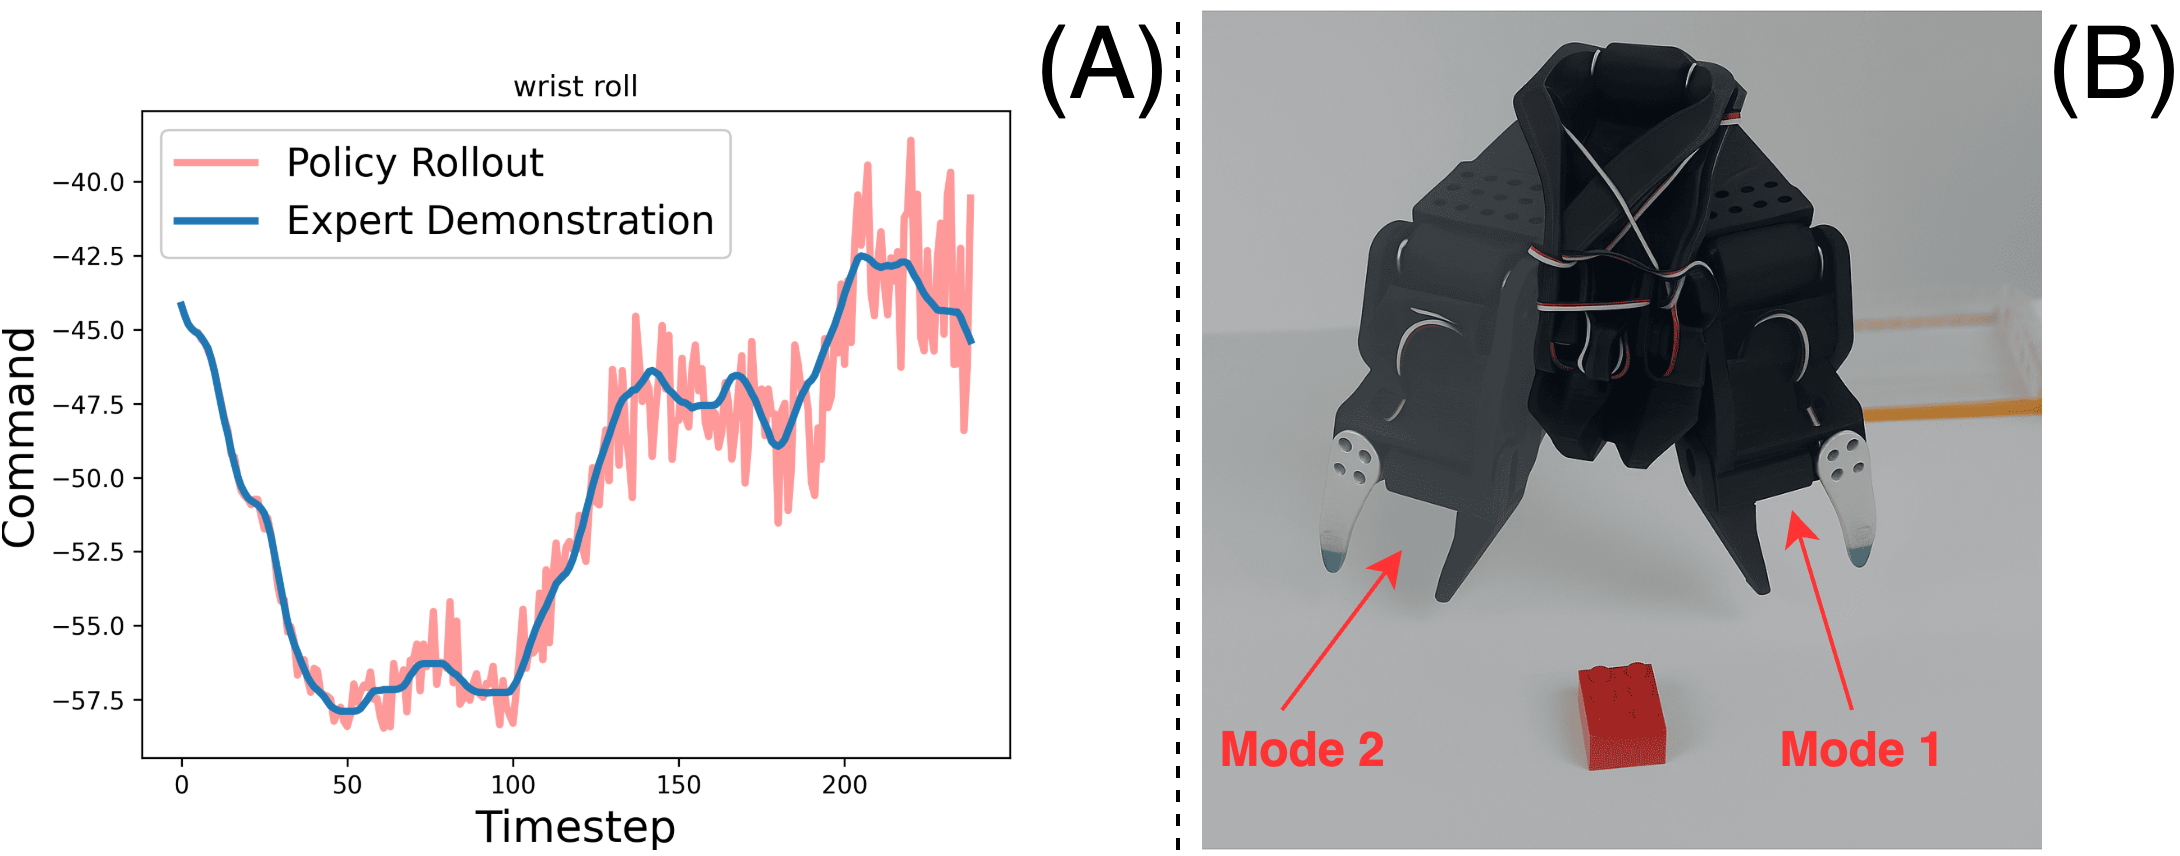
\includegraphics[width=\linewidth,height=0.62\textheight,keepaspectratio]{ch4/ch4-issues-with-bc.png}
  \begin{itemize}
    \item \highlight{Covariate shift}: small errors push the policy out of the demo distribution.
    \item \highlight{Multimodality}: averaging over several valid strategies yields indecisive actions.
  \end{itemize}
  \sources{\citep{rossReductionImitationLearning2011,florenceImplicitBehavioralCloning2022,keGraspingChopsticksCombating2020}}
\end{frame}

\begin{frame}{Why Generative Models Help}
  \begin{itemize}
    \item Instead of predicting one best action, learn a \highlight{distribution} over valid actions.
    \item That is exactly what you want when the same task admits multiple successful behaviors.
    \item In this chapter, generative models become the main tool for modeling rich action distributions.
  \end{itemize}
\end{frame}

\begin{frame}{VAE Intuition: A Latent for Behavior}
  \begin{columns}[T,onlytextwidth]
    \begin{column}{0.52\textwidth}
      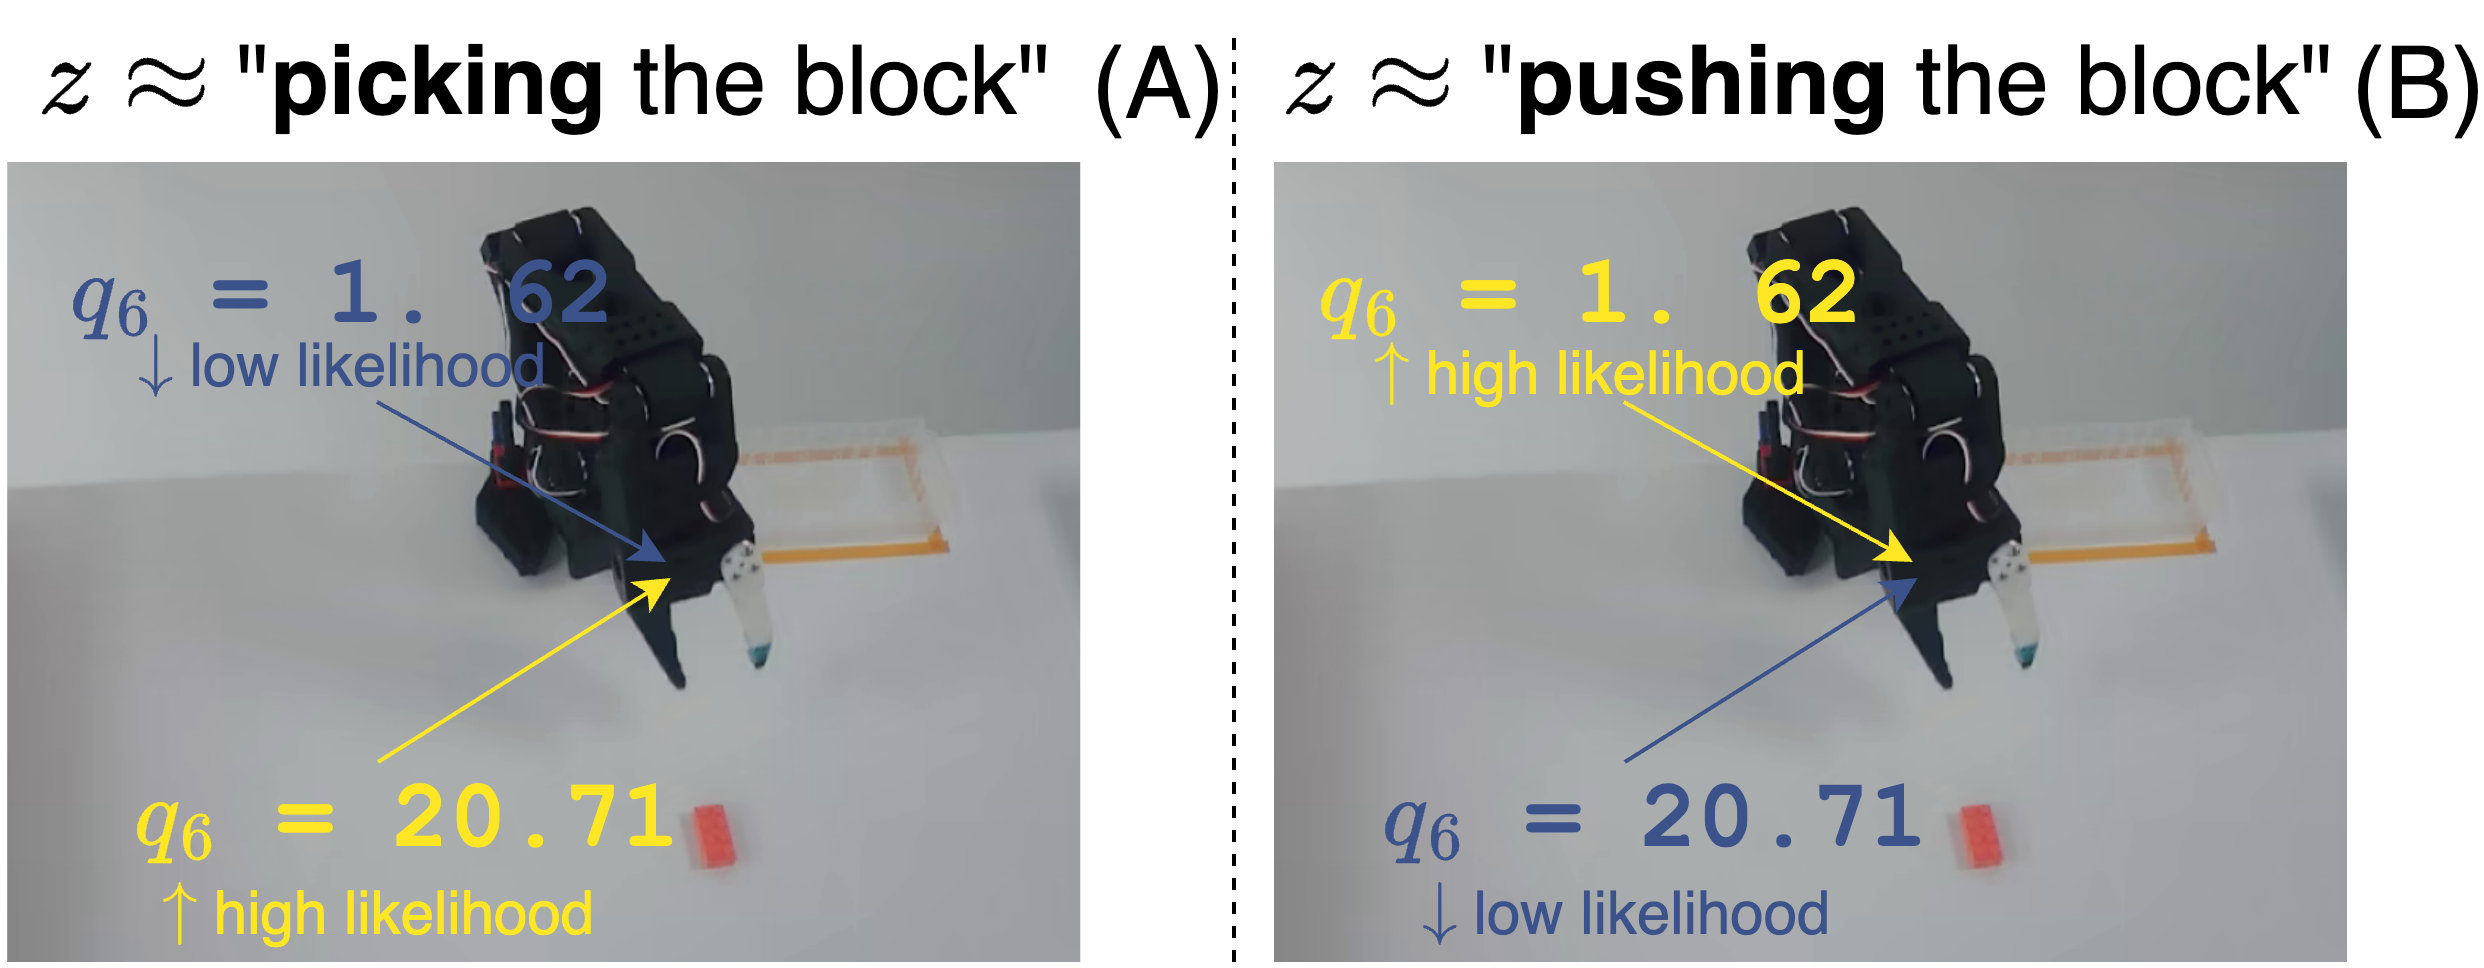
\includegraphics[width=\linewidth]{ch4/ch4-task-effect-on-pairs.png}
    \end{column}
    \begin{column}{0.44\textwidth}
      \begin{itemize}
        \item A latent variable \(z\) can encode task style or strategy.
        \item VAEs reconstruct samples while regularizing the latent space.
        \item Conditional VAEs are especially useful when actions must be generated \highlight{given observations}.
      \end{itemize}
    \end{column}
  \end{columns}
\end{frame}

\begin{frame}{Diffusion: Learn to Denoise Action Distributions}
  \begin{columns}[T,onlytextwidth]
    \begin{column}{0.48\textwidth}
      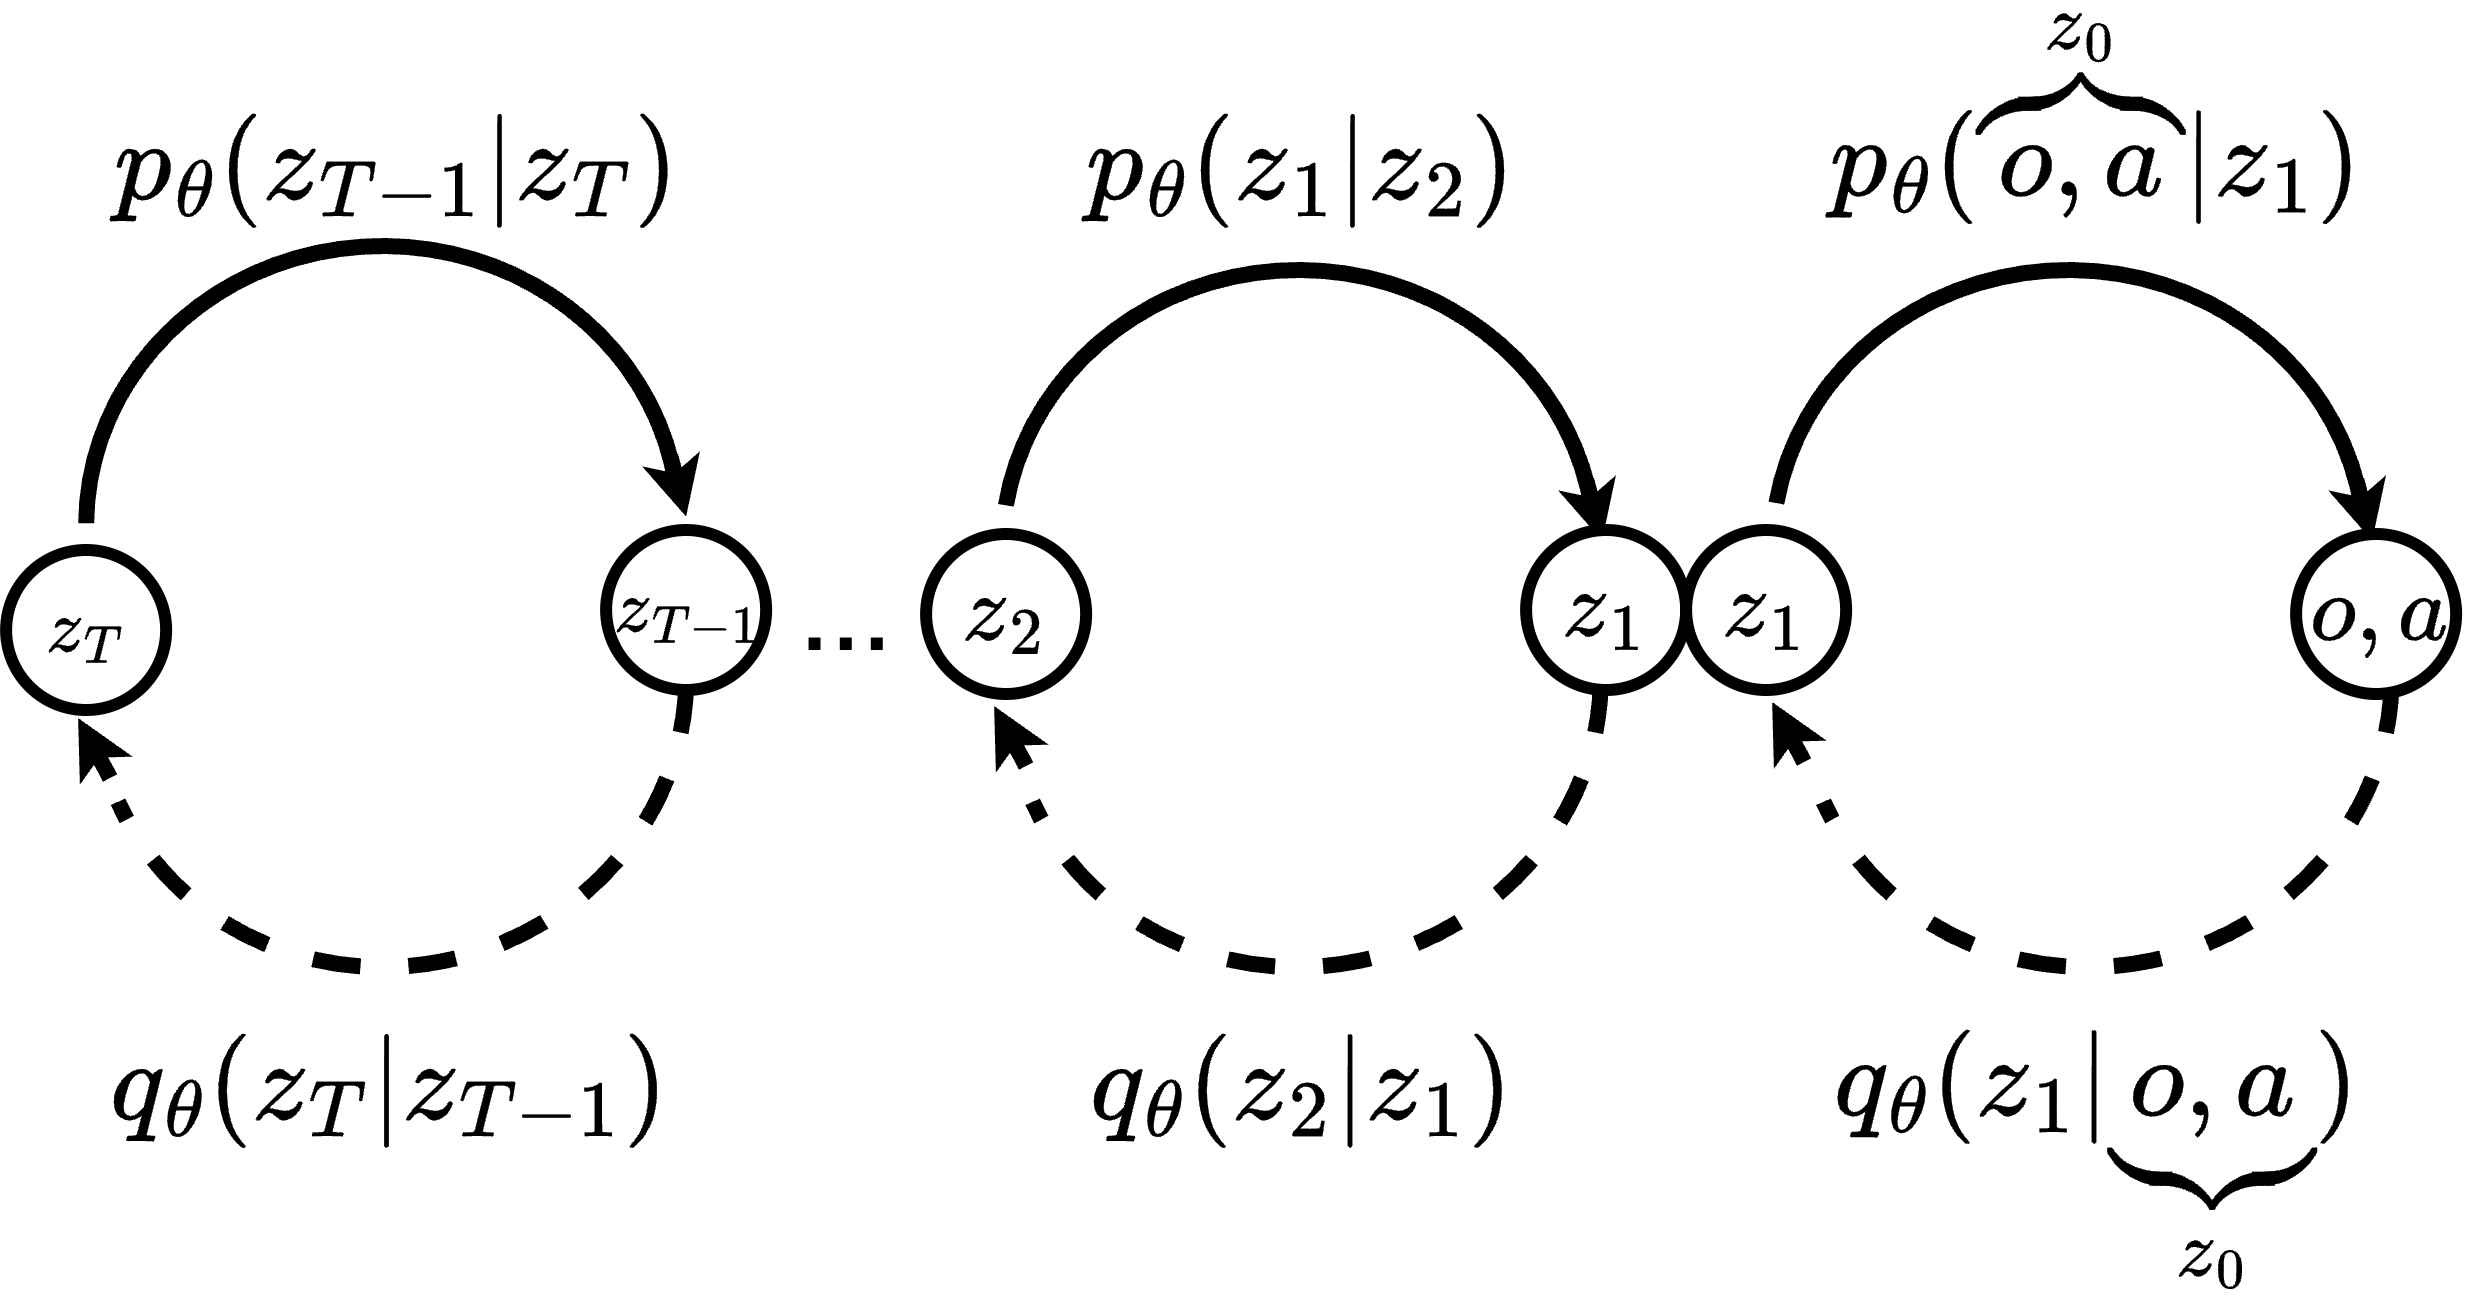
\includegraphics[width=\linewidth,height=0.38\textheight,keepaspectratio]{ch4/ch4-many-latents.png}
    \end{column}
    \begin{column}{0.48\textwidth}
      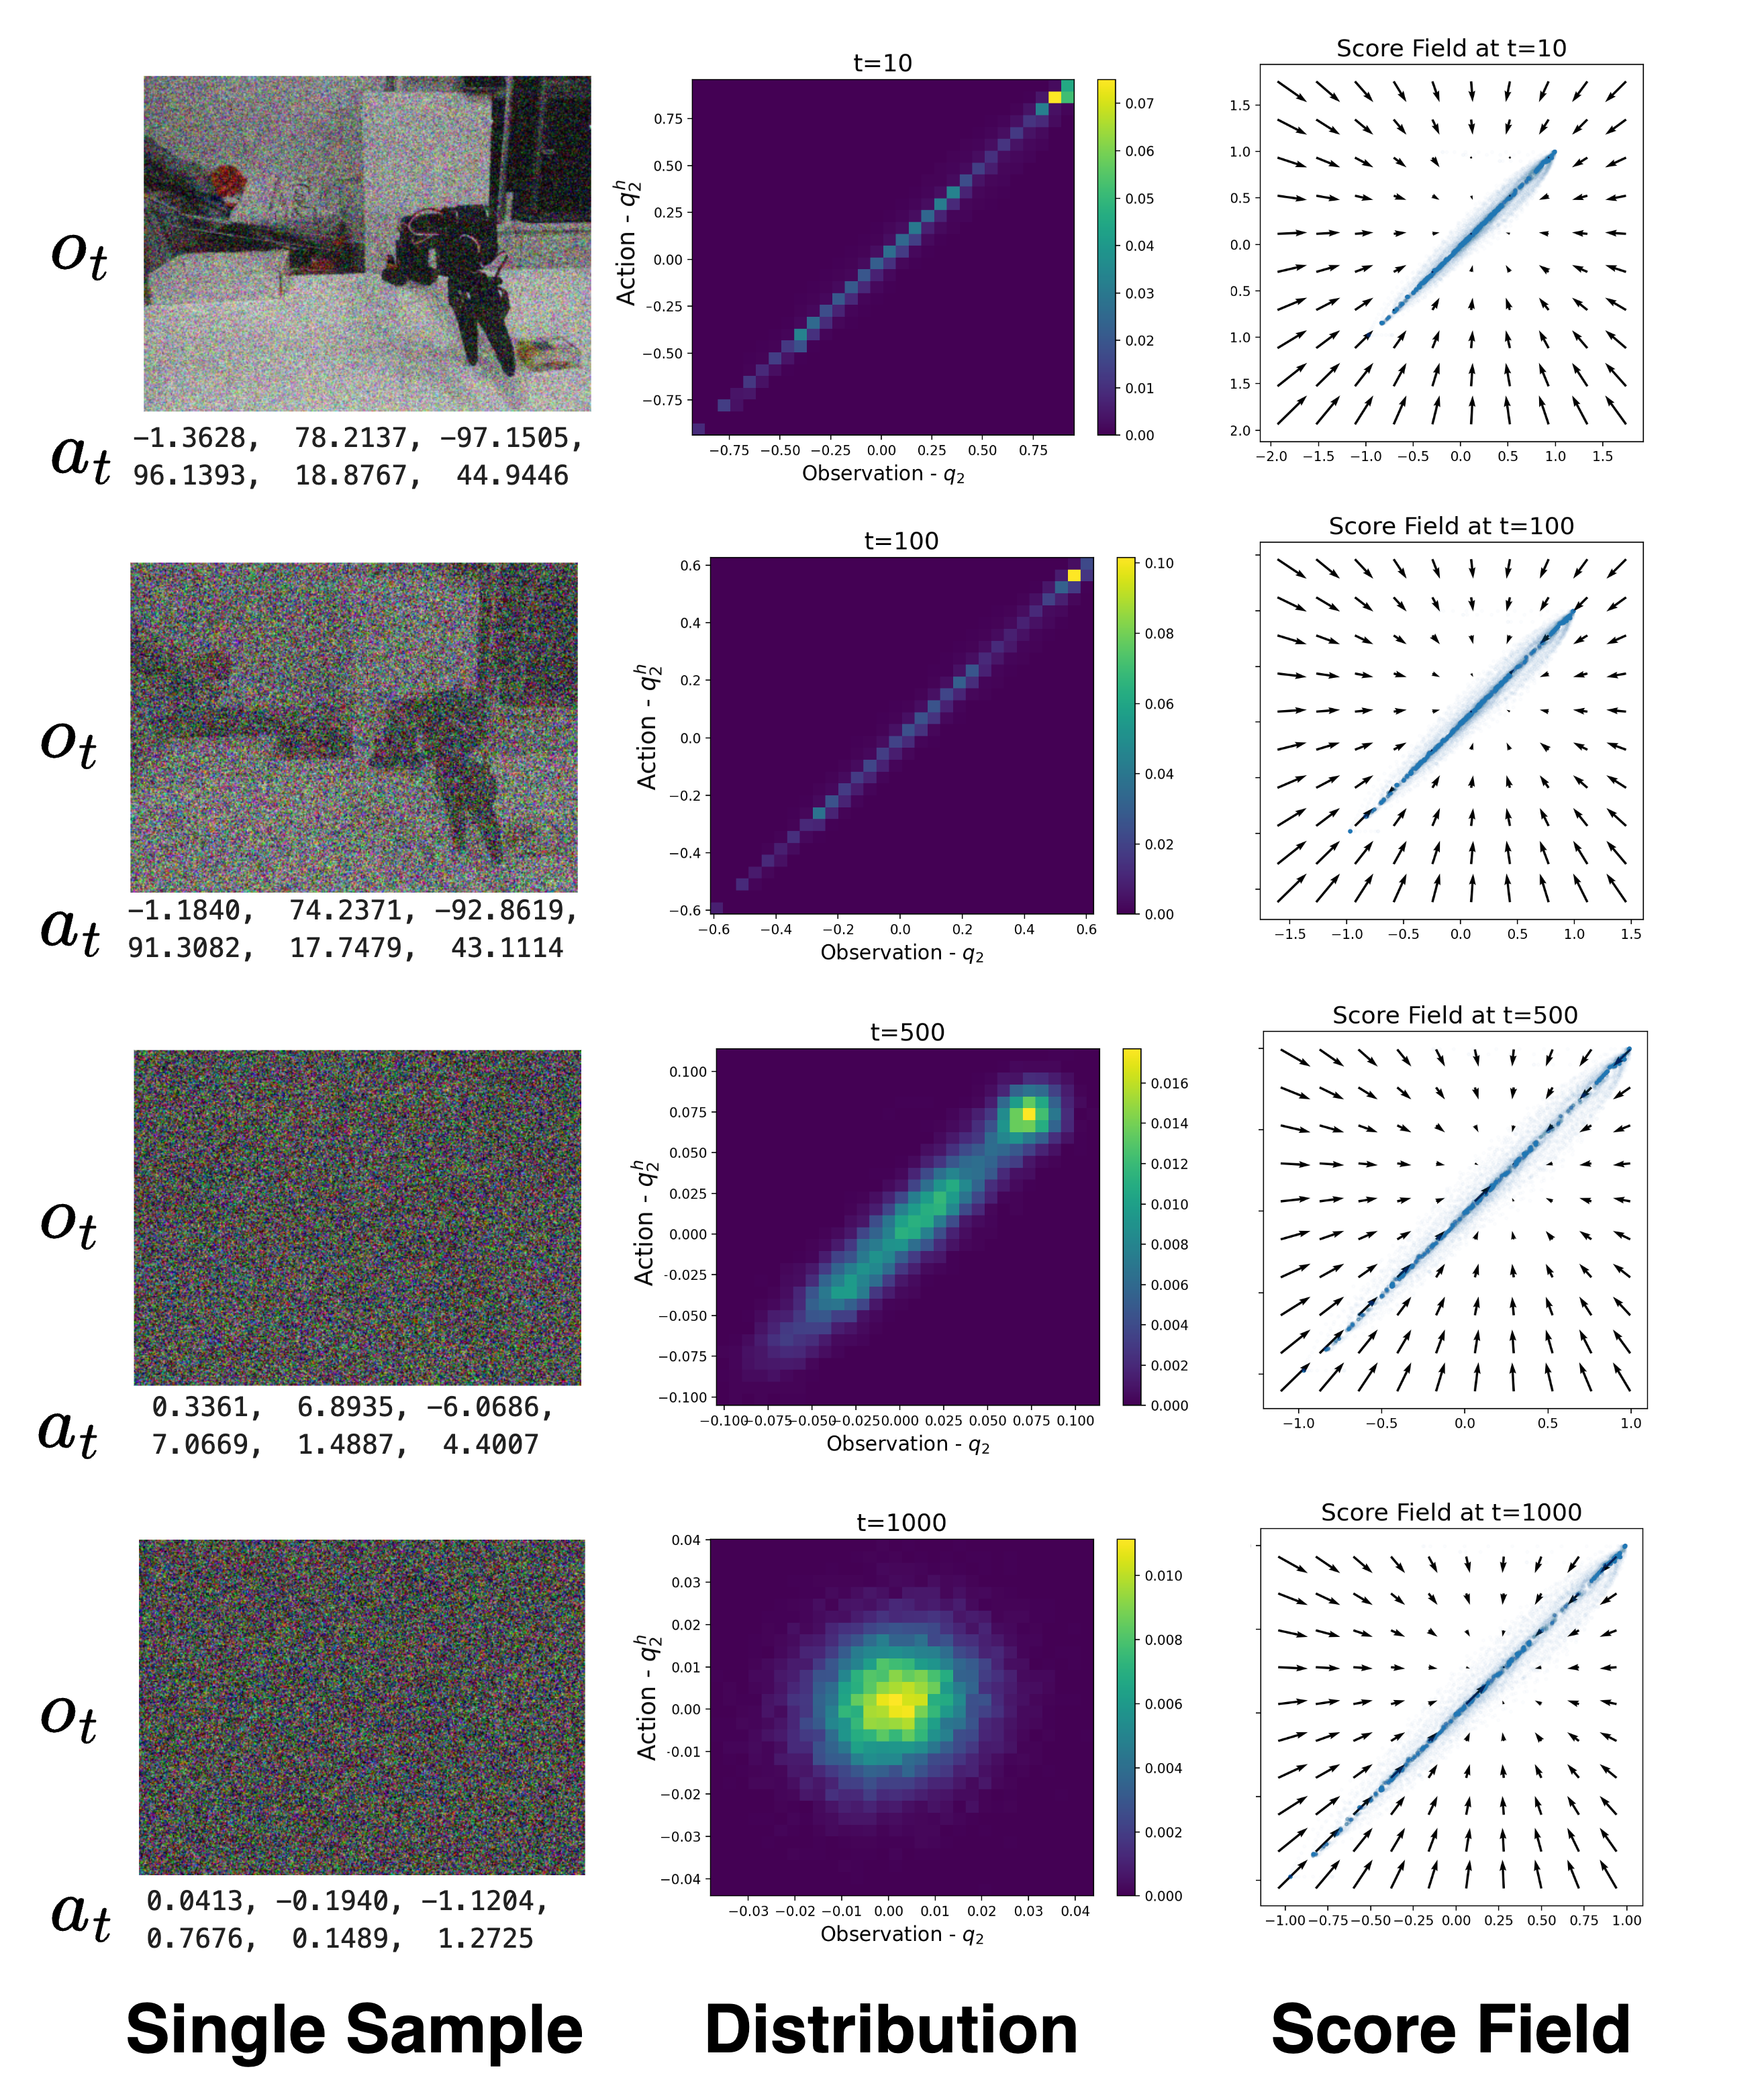
\includegraphics[width=\linewidth,height=0.38\textheight,keepaspectratio]{ch4/ch4-diffusion-robot-actions.png}
    \end{column}
  \end{columns}

  \vspace{0.2cm}
  \begin{itemize}
    \item Corrupt data toward noise, then learn to reverse that corruption.
    \item The denoising process naturally models \highlight{high-dimensional, multimodal} targets.
  \end{itemize}
  \sources{\citep{hoDenoisingDiffusionProbabilistic2020,permenterInterpretingImprovingDiffusion2024}}
\end{frame}

\begin{frame}{Flow Matching: Straighter Paths, Faster Inference}
  \begin{columns}[T,onlytextwidth]
    \begin{column}{0.5\textwidth}
      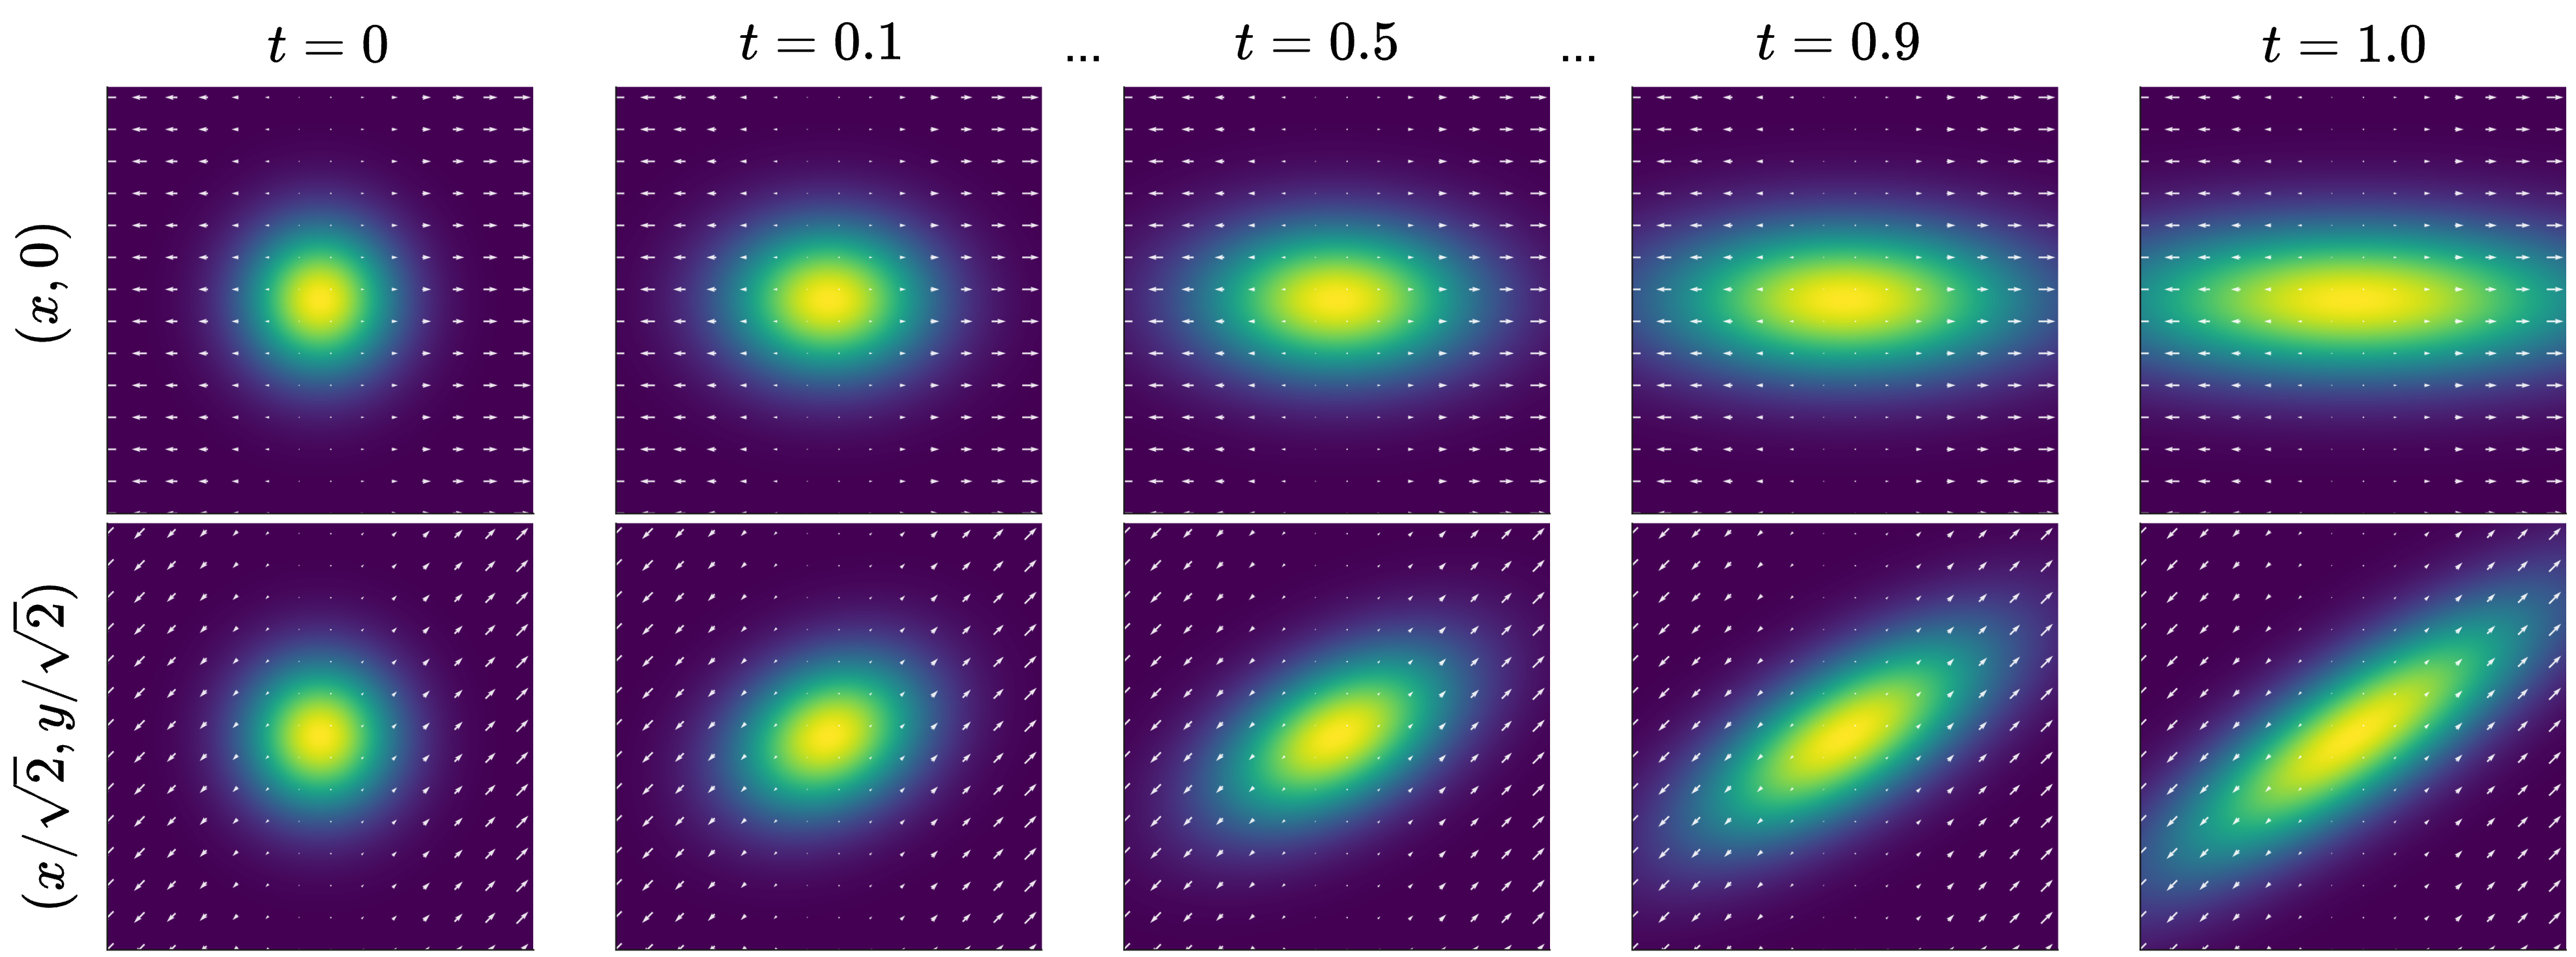
\includegraphics[width=\linewidth]{ch4/ch4-normalizing-flows.png}
    \end{column}
    \begin{column}{0.46\textwidth}
      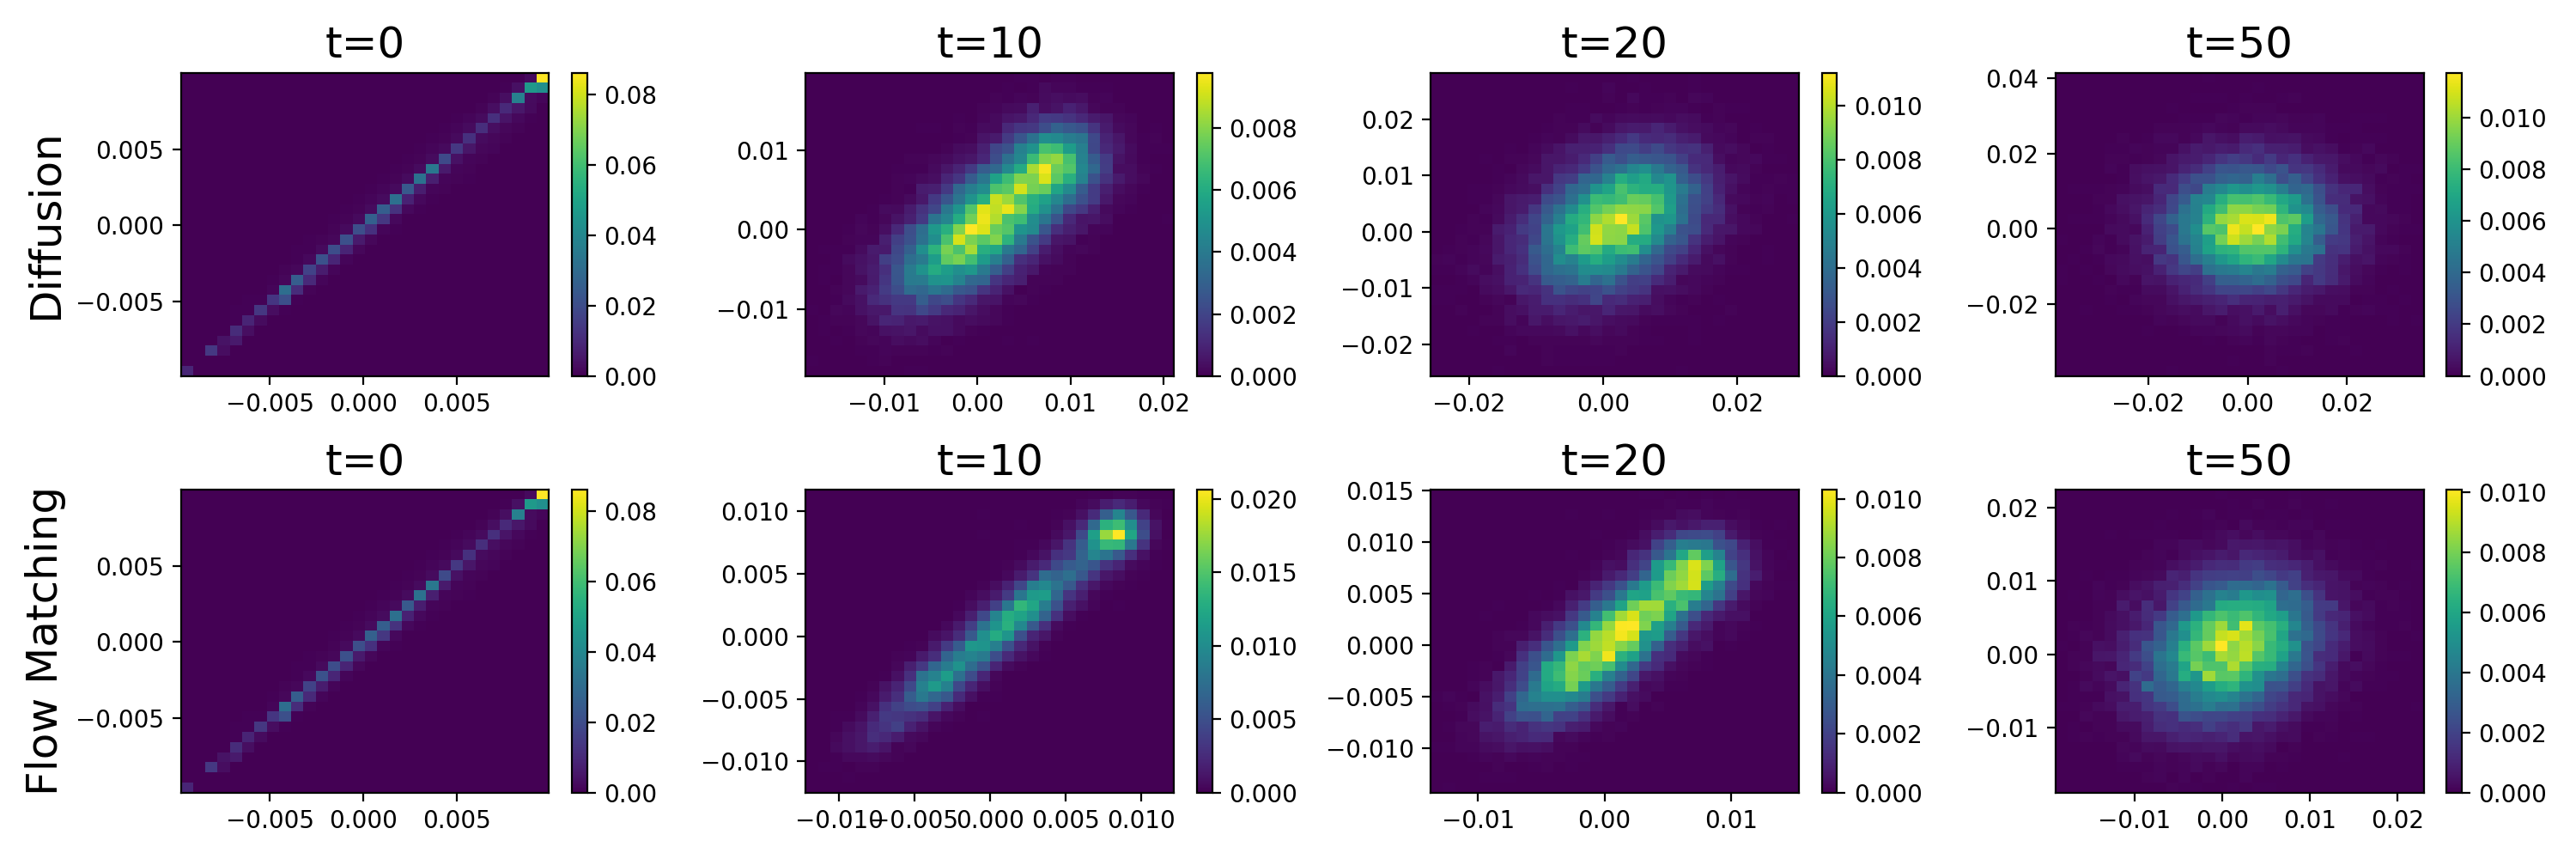
\includegraphics[width=\linewidth]{ch4/ch4-diffusion-vs-flowmatching.png}
    \end{column}
  \end{columns}

  \vspace{0.2cm}
  \begin{itemize}
    \item Flow matching learns a continuous vector field instead of a long stochastic denoising chain.
    \item That usually means \highlight{fewer integration steps} at inference time.
  \end{itemize}
  \sources{\citep{lipmanFlowMatchingGenerative2023,esserScalingRectifiedFlow2024}}
\end{frame}

\begin{frame}{ACT: Predict Action Chunks, Not Single Actions}
  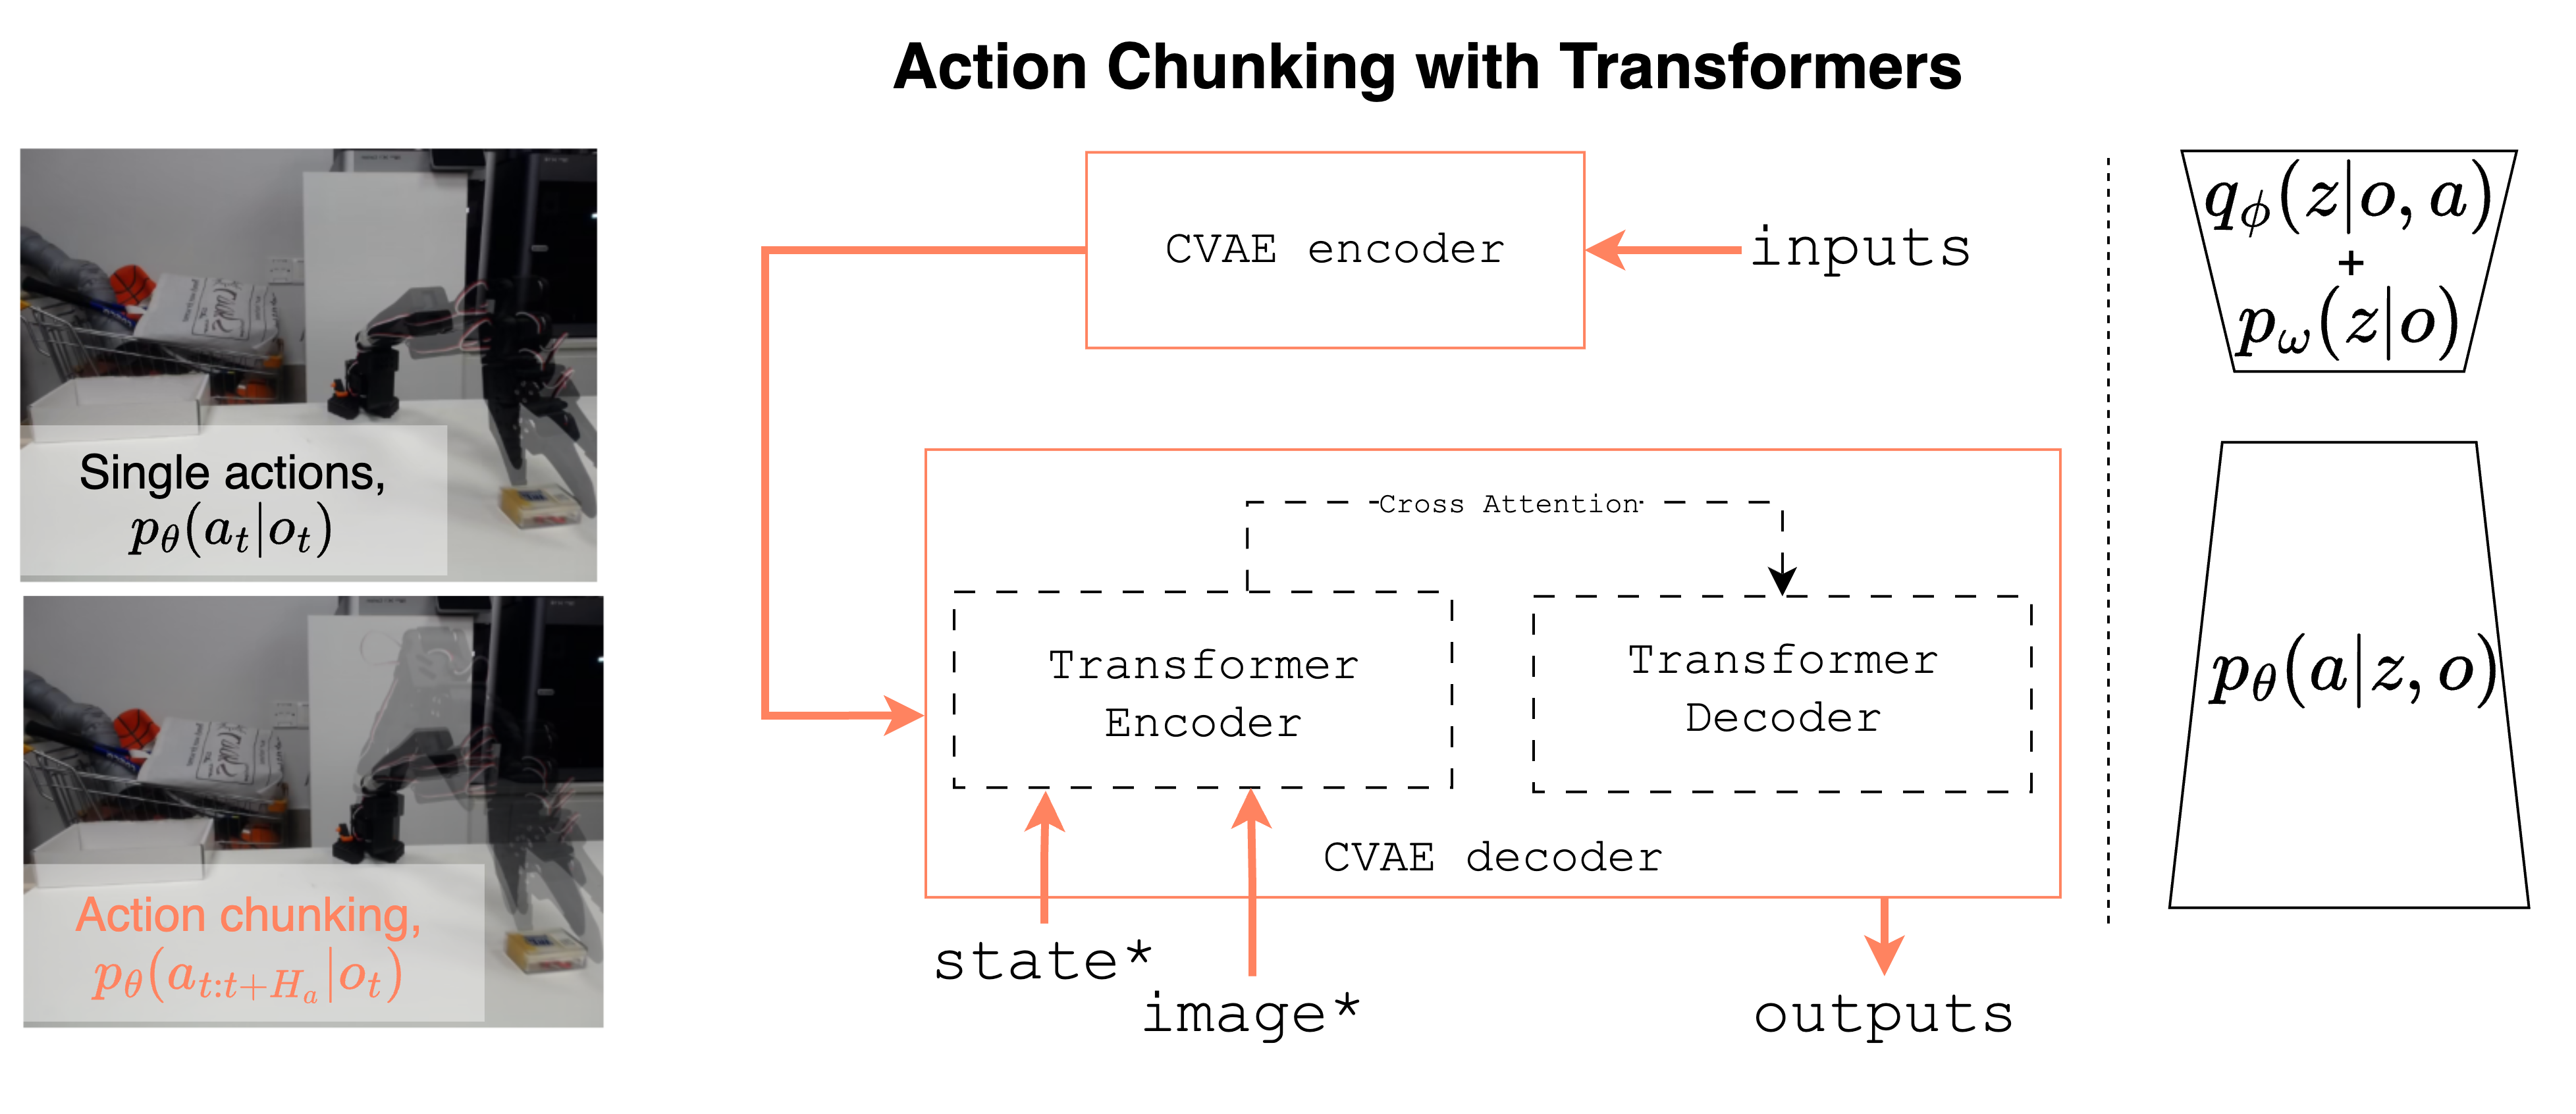
\includegraphics[width=\linewidth,height=0.62\textheight,keepaspectratio]{ch4/ch4-act.png}
  \begin{itemize}
    \item ACT uses a transformer-based conditional VAE and predicts future \highlight{chunks of actions}.
    \item Chunking reduces compounding errors and helps the policy commit to coherent behavior.
  \end{itemize}
  \sources{\citep{zhaoLearningFineGrainedBimanual2023}}
\end{frame}

\begin{frame}{ACT Encoder}
  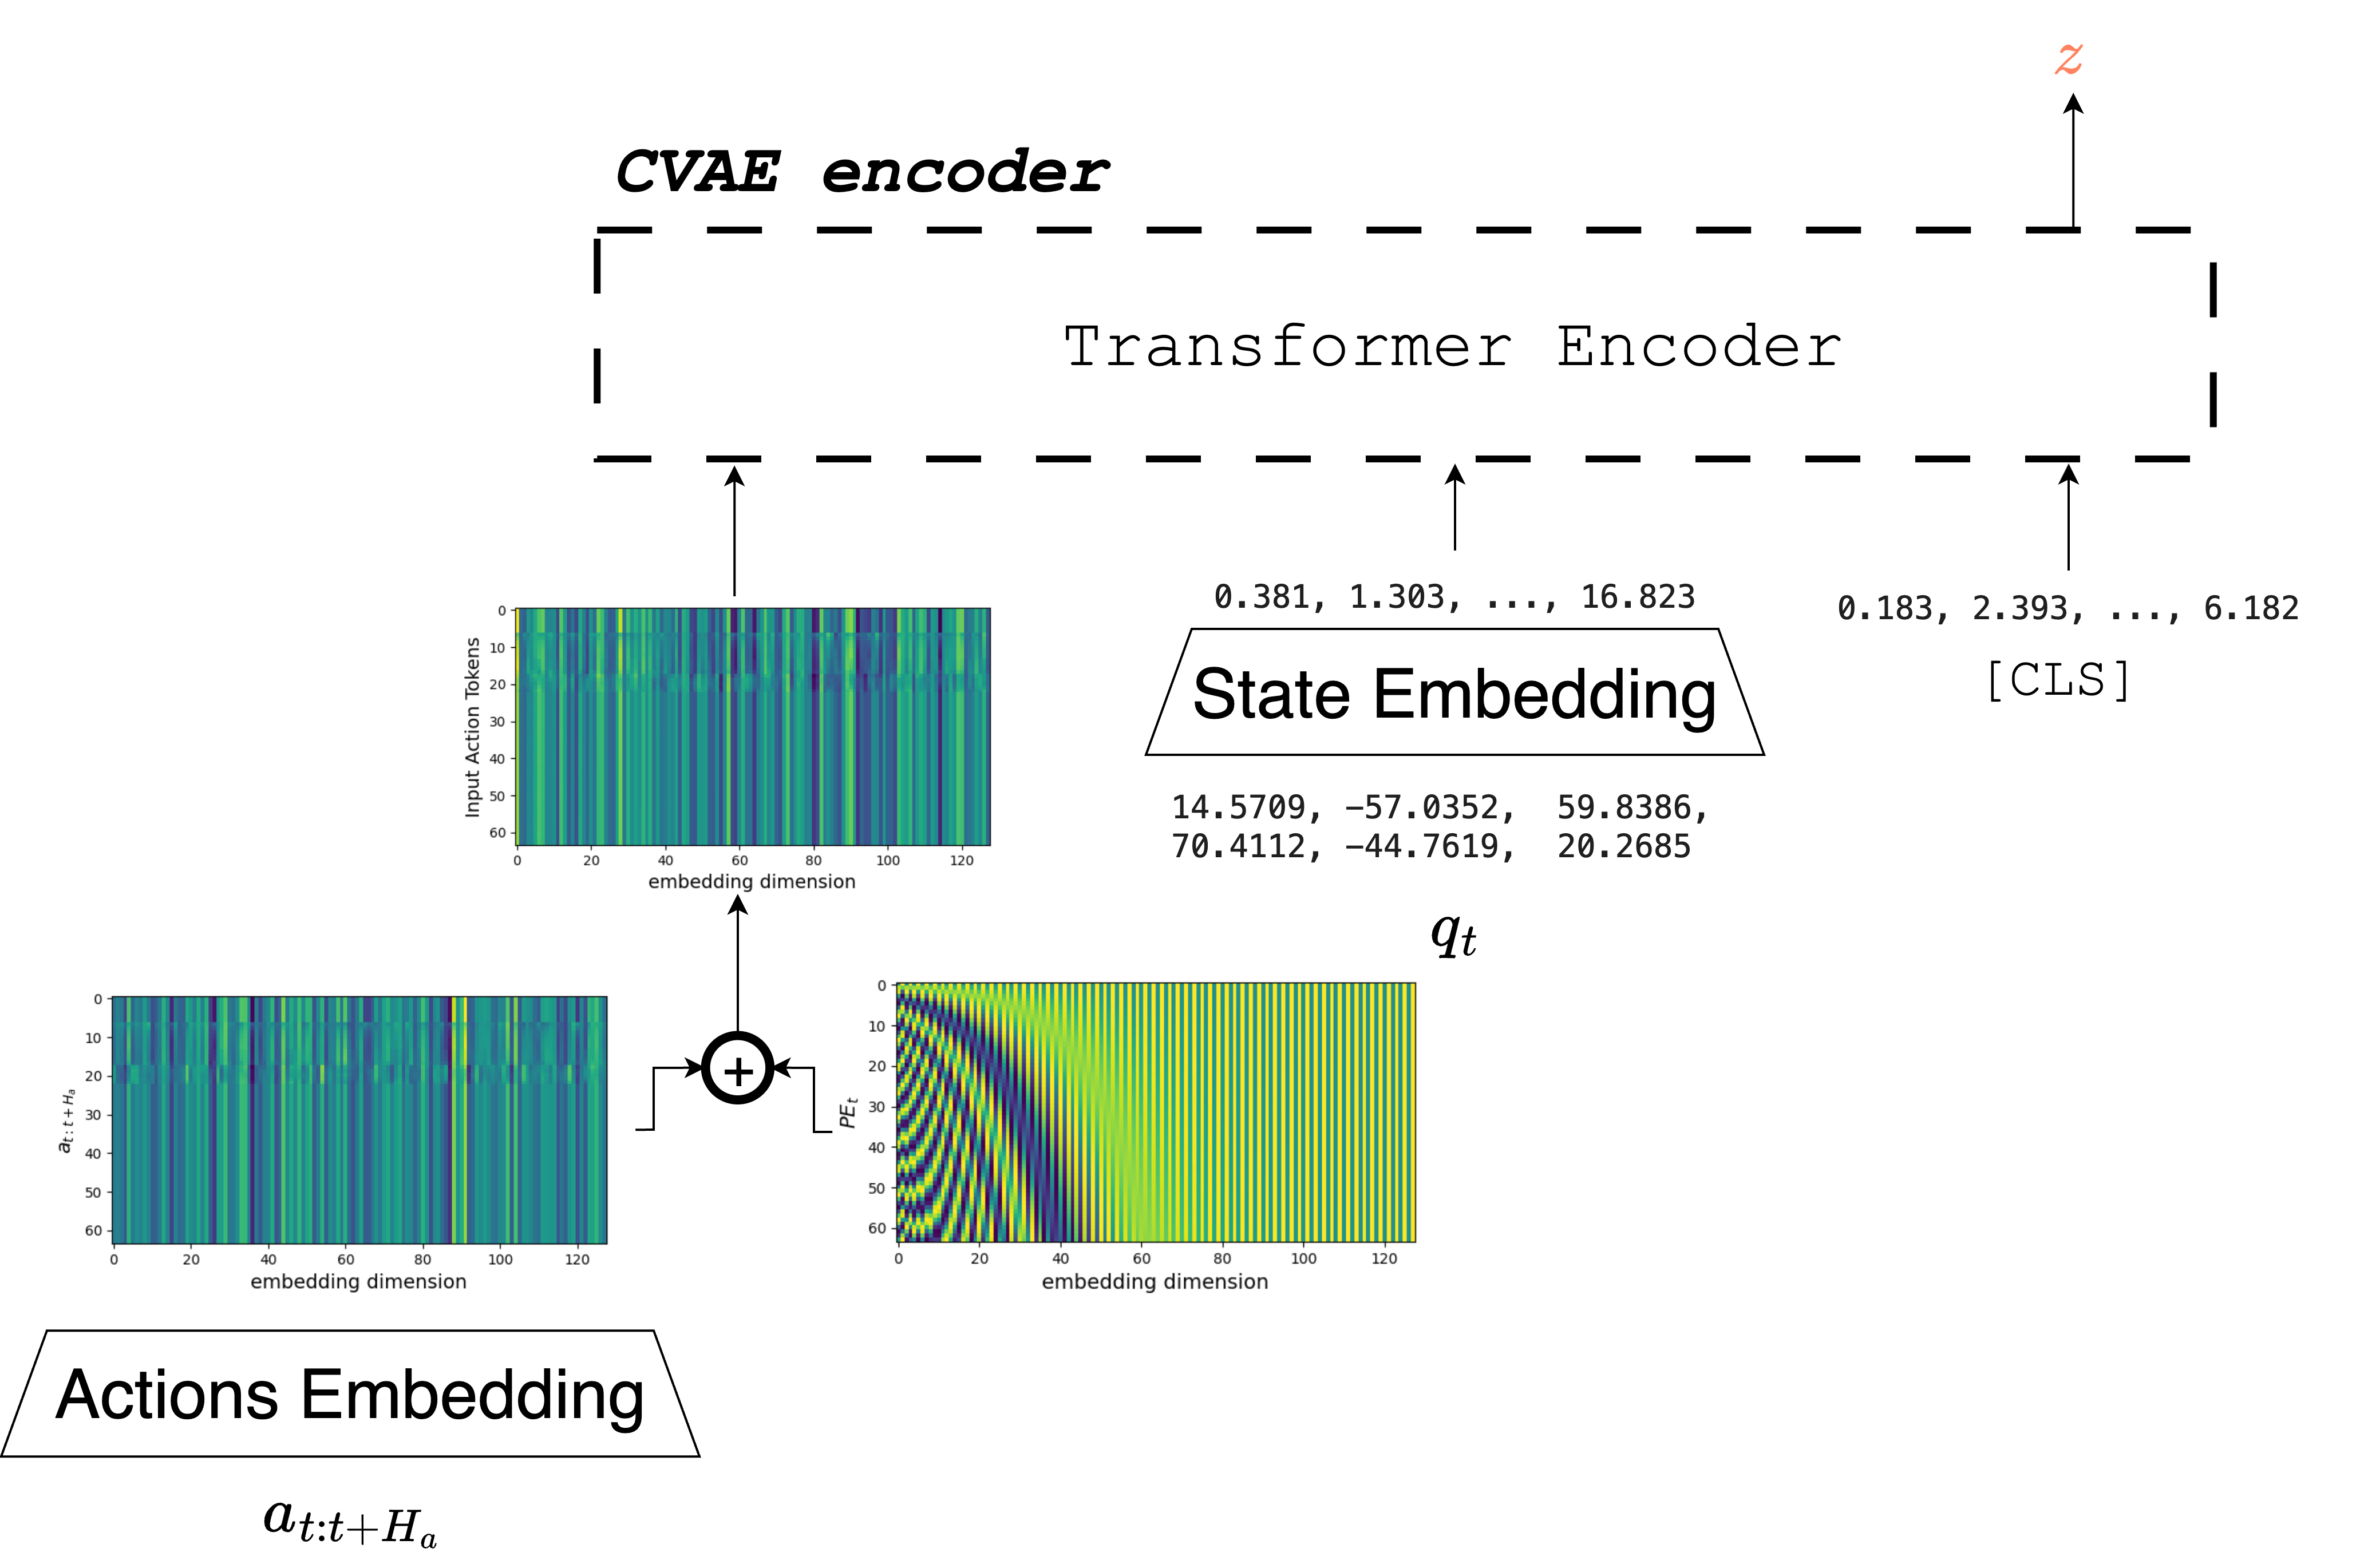
\includegraphics[width=\linewidth,height=0.64\textheight,keepaspectratio]{ch4/ch4-act-encoder.png}

  \begin{itemize}
    \item The encoder is a \highlight{training-time} component used to infer the latent style variable from action chunks and proprioception.
    \item It teaches the decoder a richer latent structure than plain supervised regression.
  \end{itemize}
\end{frame}

\begin{frame}{ACT Decoder}
  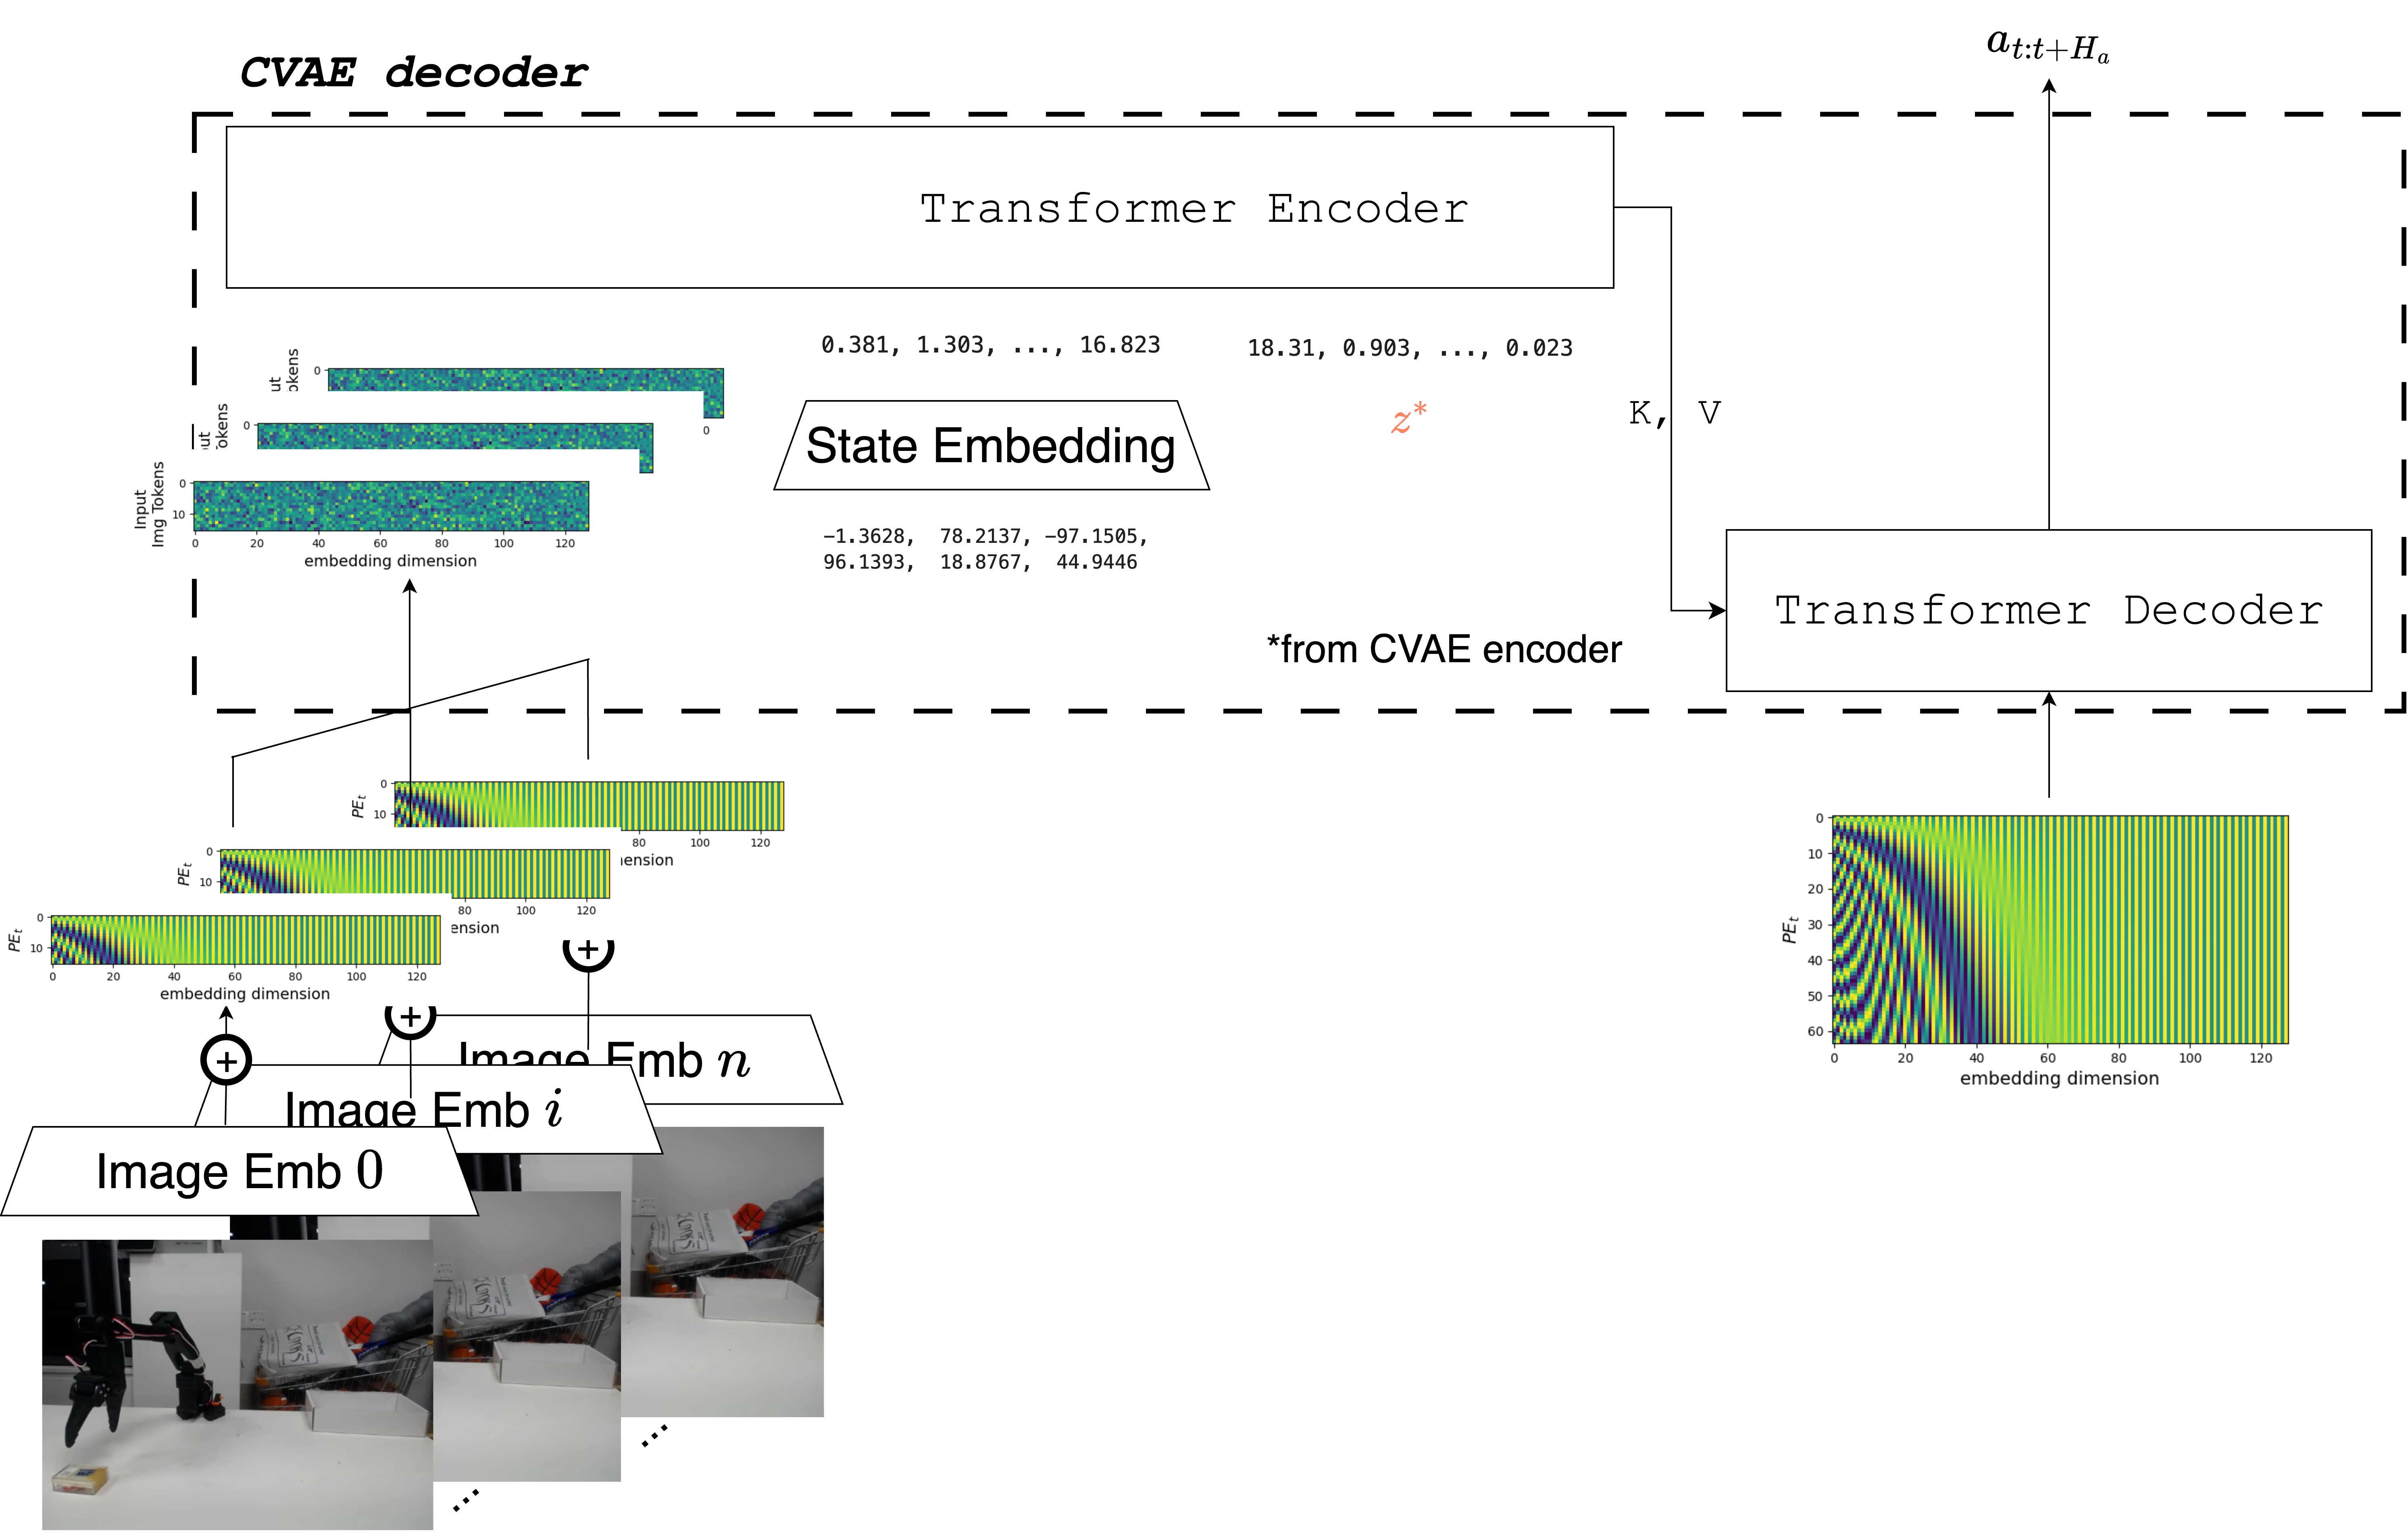
\includegraphics[width=\linewidth,height=0.64\textheight,keepaspectratio]{ch4/ch4-act-decoder.png}

  \begin{itemize}
    \item The decoder combines image features, proprioception, and the latent variable to generate an action chunk.
    \item At inference, ACT uses a deterministic latent choice and relies on this decoder to turn observations into coherent behavior.
  \end{itemize}
\end{frame}

\begin{frame}{ACT in Practice}
  \begin{block}{Reference snippets}
    \texttt{snippets/ch4/01\_training\_act.py} and \texttt{snippets/ch4/02\_using\_act.py}
  \end{block}

  \begin{itemize}
    \item Train a chunk-predicting policy from offline demonstrations.
    \item Use chunk overlap aggregation at inference to avoid fully open-loop execution.
  \end{itemize}
\end{frame}

\begin{frame}{Diffusion Policy}
  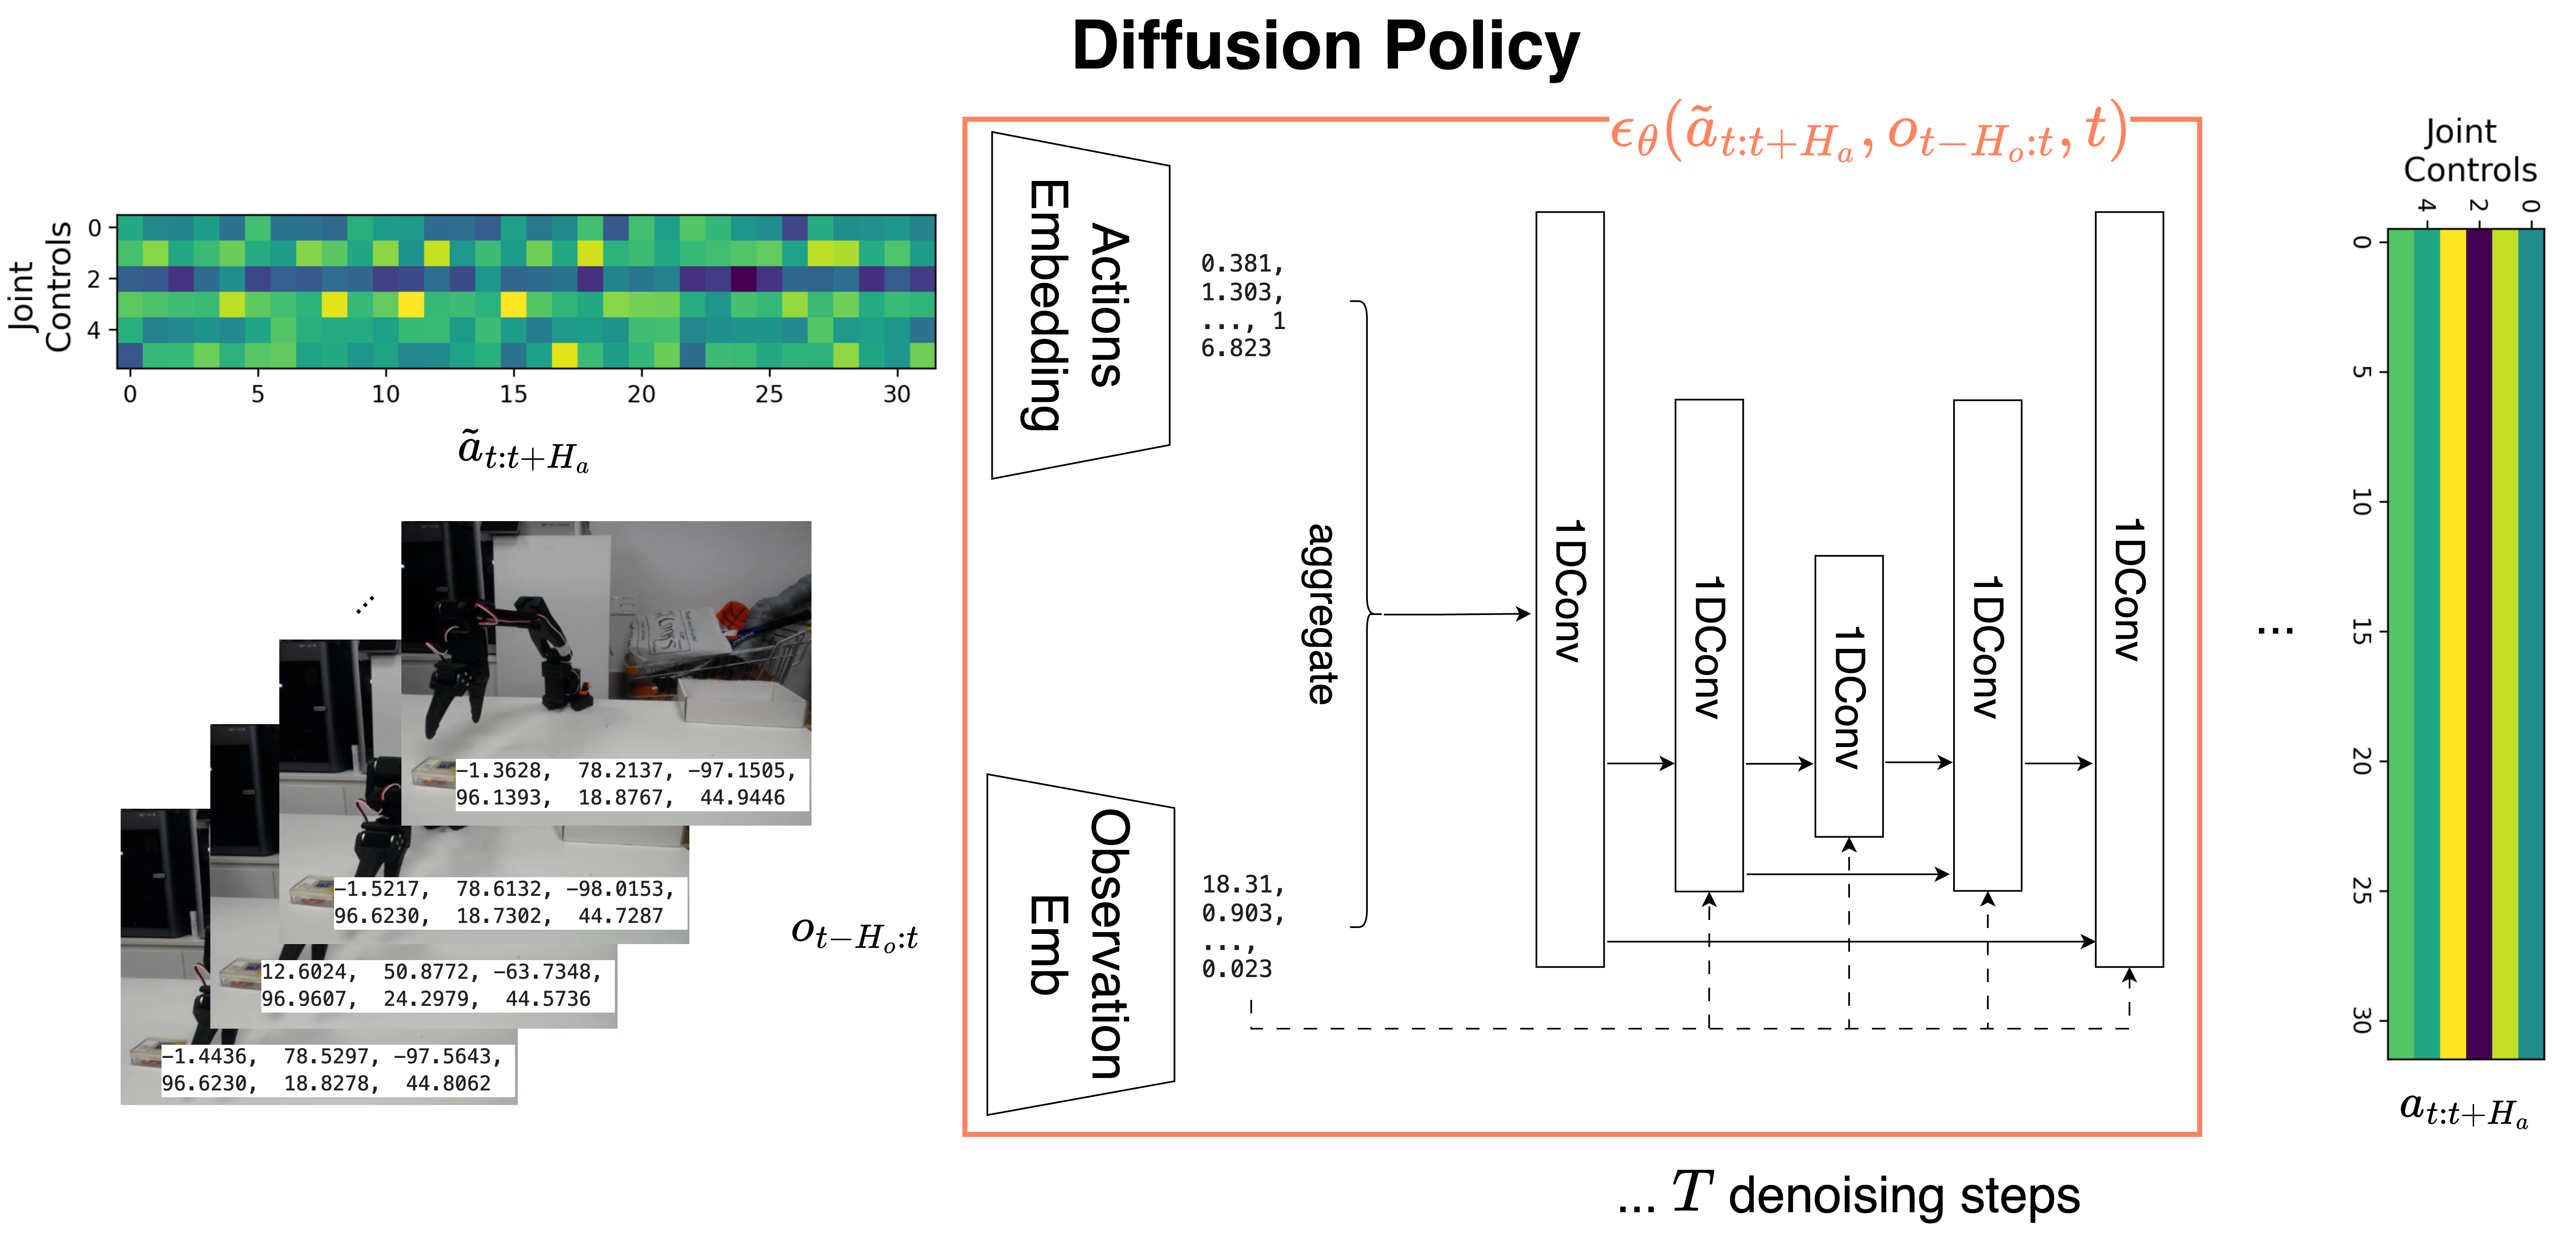
\includegraphics[width=\linewidth,height=0.58\textheight,keepaspectratio]{ch4/ch4-diffusion-policy.png}
  \begin{itemize}
    \item Diffusion Policy conditions on a history of observations and denoises a future action chunk.
    \item Conditioning on observations and predicting multiple actions helps the model \highlight{commit to a mode} of behavior.
  \end{itemize}
  \sources{\citep{chiDiffusionPolicyVisuomotor2024,hoDenoisingDiffusionProbabilistic2020,songDenoisingDiffusionImplicit2022}}
\end{frame}

\begin{frame}{Diffusion Policy in Practice}
  \begin{itemize}
    \item Works with surprisingly small real-world datasets: tens to low hundreds of demonstrations.
    \item Uses a conditional denoising objective rather than reconstructing observations themselves.
    \item Reference snippets:
    \item \texttt{snippets/ch4/03\_training\_diffusion.py}
    \item \texttt{snippets/ch4/04\_using\_diffusion.py}
  \end{itemize}
\end{frame}

\begin{frame}{Asynchronous Inference}
  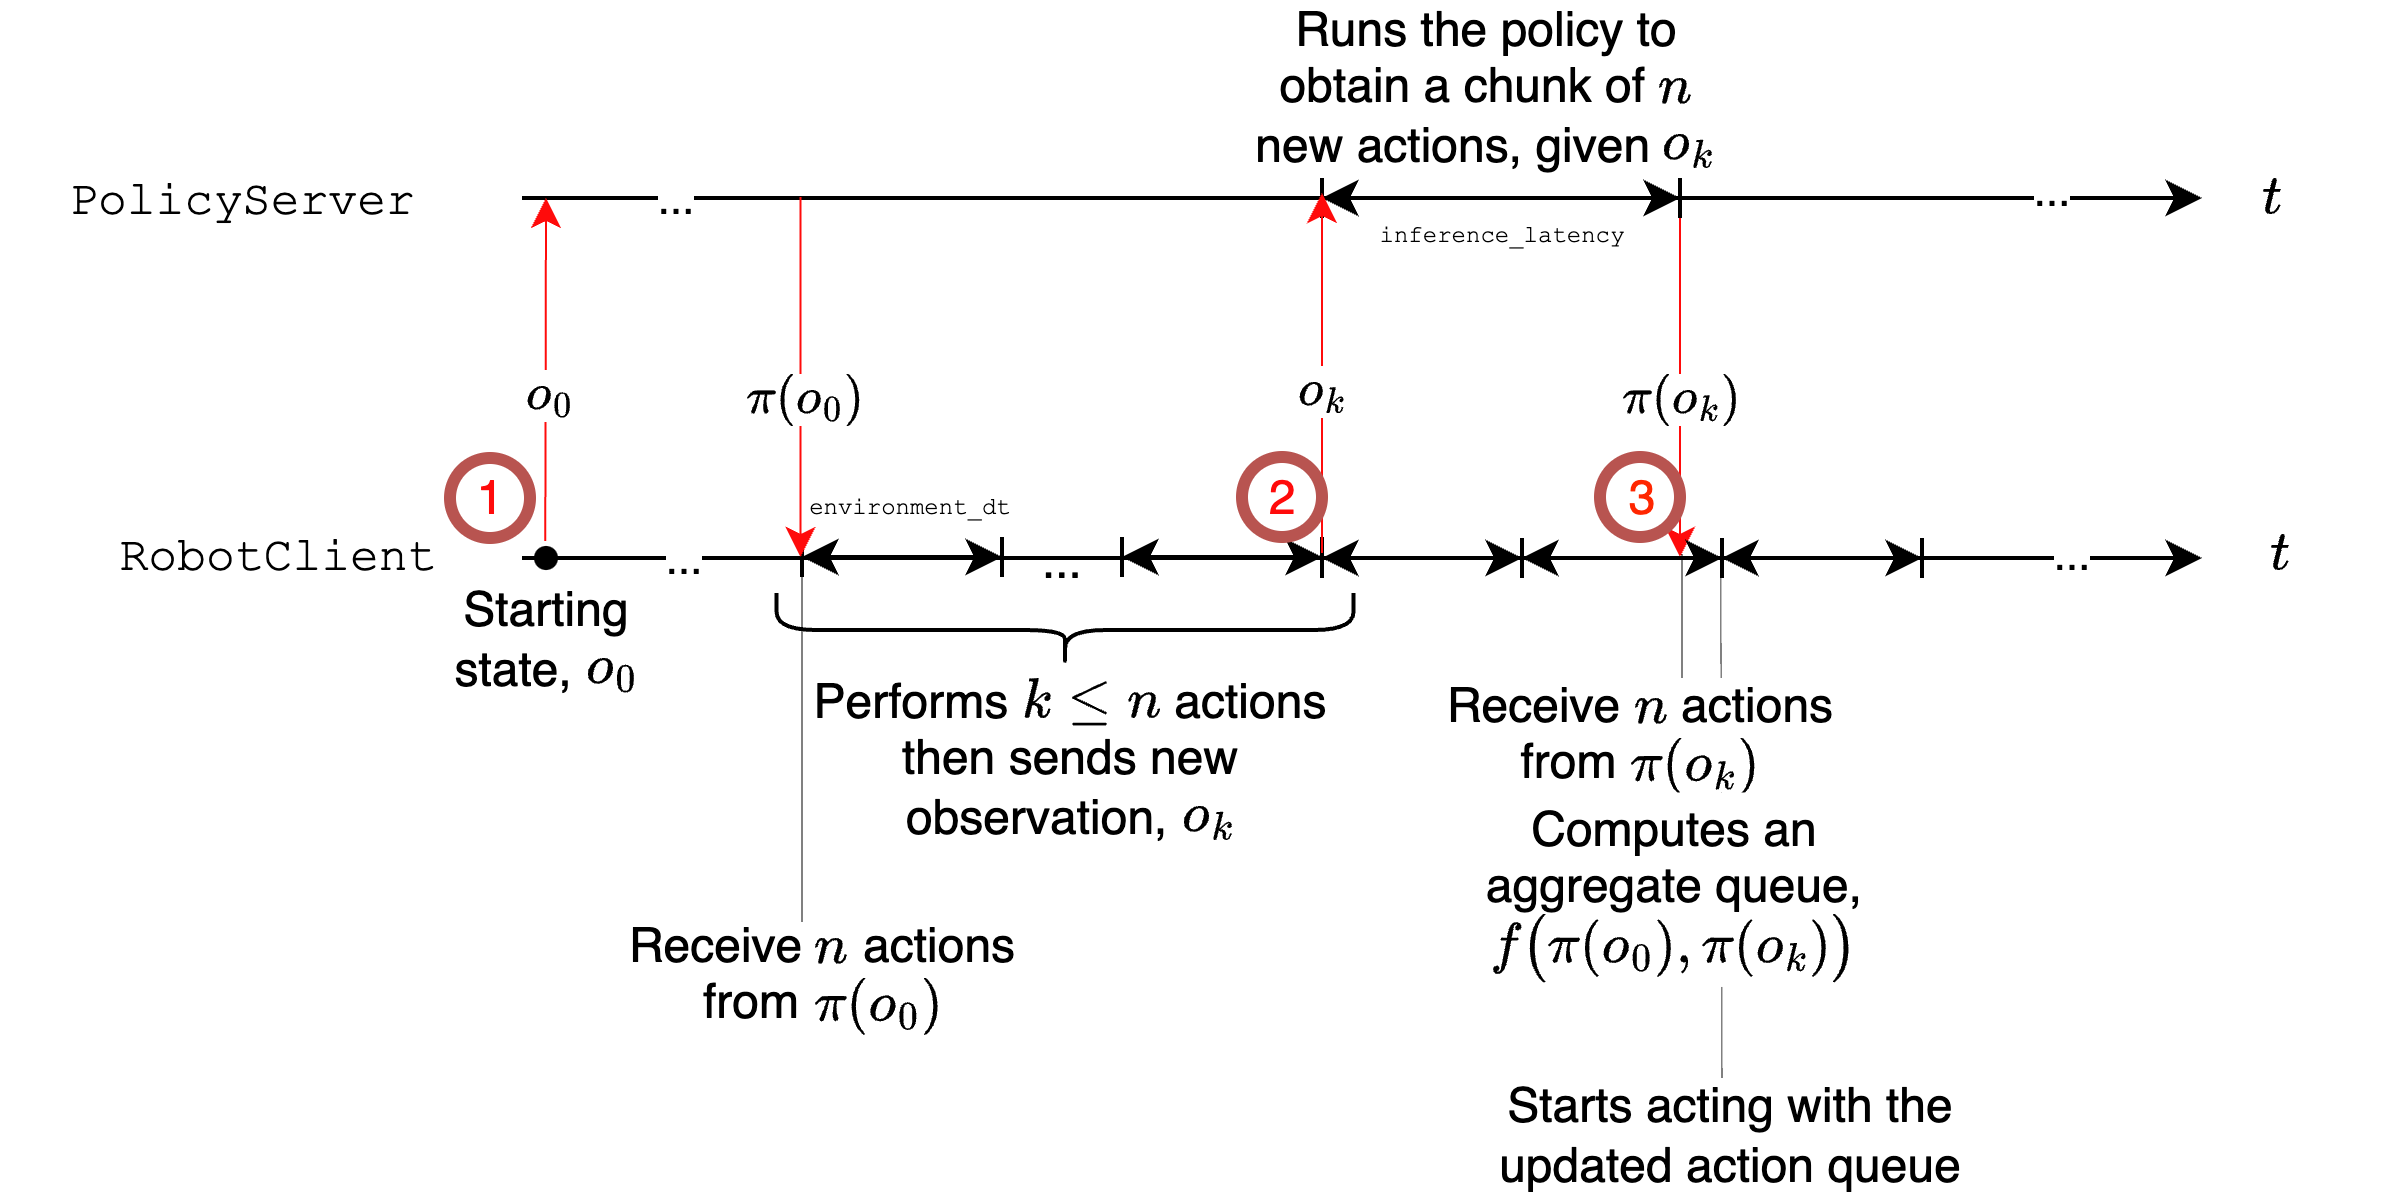
\includegraphics[width=\linewidth,height=0.62\textheight,keepaspectratio]{ch4/ch4-async-inference.png}
  \begin{itemize}
    \item Predicting action chunks creates a systems opportunity: \highlight{separate chunk prediction from action execution}.
    \item A robot client can keep executing while a local or remote policy server computes the next chunk.
  \end{itemize}
  \sources{\citep{zhaoLearningFineGrainedBimanual2023}}
\end{frame}

\begin{frame}{Choosing the Queue Overlap}
  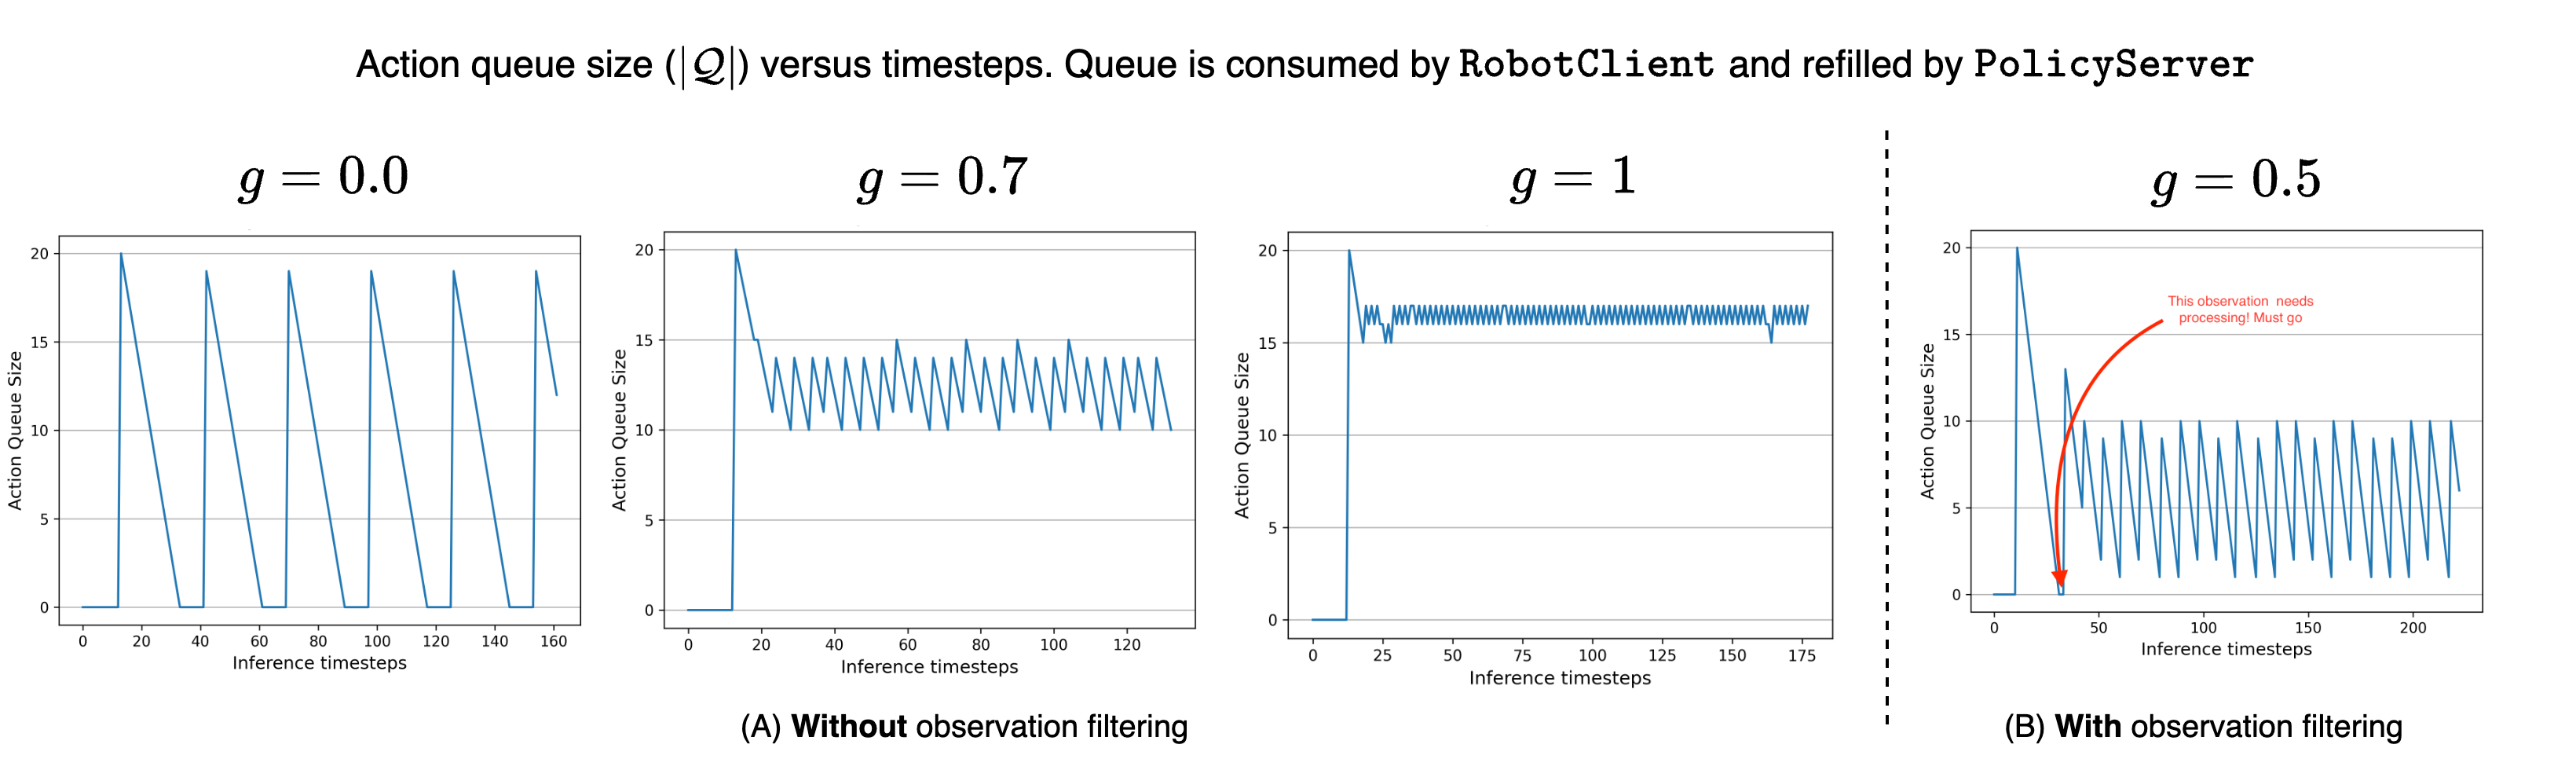
\includegraphics[width=\linewidth,height=0.62\textheight,keepaspectratio]{ch4/ch4-queues.png}
  \begin{itemize}
    \item Small overlap means idle gaps.
    \item Large overlap means more compute and more frequent policy calls.
    \item The threshold \(g\) controls the responsiveness-versus-cost tradeoff.
  \end{itemize}
\end{frame}

\begin{frame}{Deploying Async Inference}
  \begin{block}{Reference snippets}
    \texttt{snippets/ch4/05\_policy\_server.py} and \texttt{snippets/ch4/06\_robot\_client.py}
  \end{block}

  \begin{itemize}
    \item Run the policy server on stronger hardware if needed.
    \item Filter near-duplicate observations to avoid redundant chunk requests.
    \item Keep action execution smooth while still reacting to fresh observations.
  \end{itemize}
\end{frame}

\begin{frame}{Chapter Takeaway}
  \begin{itemize}
    \item BC becomes much stronger when actions are modeled as \highlight{distributions}, not point estimates.
    \item Chunked generative policies like ACT and Diffusion Policy are a practical response to multimodality and sequential error compounding.
    \item Once chunk prediction exists, deployment strategy matters almost as much as model architecture.
  \end{itemize}
\end{frame}

\begin{frame}[allowframebreaks]{Selected References}
\scriptsize
\nocite{pomerleauALVINNAutonomousLand1988}
\bibliography{../shared/references}
\end{frame}

\end{document}
